\documentclass[oneside, noacknowlegments]{BYUPhys}
\usepackage{verbatim}
\usepackage{graphicx}
\usepackage{ragged2e}
\usepackage{amsmath}

% Your name
  \Author{Erik Swenson}

% Enter the date your thesis is approved
  \Year{2016}
  \Month{April}

% If you have a long title, split it between multiple lines using the \\ command
  \Title{Calcium and Hydrogen on Graphene as a Mechanism for 
  		 Hydrogen Storage}

% Your research advisor
\AdvisorTitle{Advisor}
  \Advisor{Bret Hess}

% For honors theses, enter the name of the honors Representative
  %\HonorsRepresentative{Kristine Hansen}

% The text of your abstract
\Abstract{ Because of its status as an emerging energy carrier, 
	methods of hydrogen storage are in high demand. Using 
	computational methods, we explore a very large space of 
	graphene structures with different adsorption configurations of 
	hydrogen and calcium as mechanisms for hydrogen storage. We 
	expand our search space further than the traditional search 
	space by using cluster expansion to enumerate structures in a 
	variety of computational cell shapes and sizes. This allows for 
	periodicities not studied previously. We also introduce 
	vacancies in the adsorption configurations and study their 
	effects. We conclude that the cell size and shape is an 
	important parameter in the search for stable structures. We 
	also find that vacancies allow for structures with more than 
	40\% calcium concentration without exhibiting signs of calcium 
	stacking. We present three stable structures that show promise 
	for hydrogen storage applications. }

 \Keywords{Hydrogen storage, cluster expansion, graphene}

% Acknowledge those who helped and supported you
  \Acknowledgments{
    [Acknowledgements should be simple, in good taste, and fit on one page]
  }

%% The members of your committee (masters only need A and B, PhD need all 4)
%  \MemberA{Committee Member A}
%  \MemberB{Committee Member B}
%  \MemberC{Committee Member C}
%  \MemberD{Committee Member D}
%

\begin{document}

 % Start page counting in roman numerals
 \frontmatter

 % This command makes the formal preliminary pages.
 % You can comment it out during the drafting process if you want to save paper.
\makepreliminarypages

% Make the table of contents.
\tableofcontents
 
% Create the list of figures.
\listoffigures

% Start regular page counting at page 1
\mainmatter

% OK. Everything is set up. Type your thesis here.

\chapter{Introduction}

\section{Motivation}
\label{sec:motivation}

In the search for lightweight, space-efficient methods of energy 
storage, molecular hydrogen has emerged as a promising energy 
carrier. New clean fuel technologies (\textit{e.g.} hydrogen fuel 
cells) take hydrogen molecules and convert the energy harnessed 
therein into some sort of fuel, usually electricity. Fuel 
technologies that utilize hydrogen energy are far less pollutant 
than standard hydrocarbon fuel sources such as gasoline or propane. 
Both production and consumption of hydrocarbon fuels can pose a 
risk to the people or the environment in densely populated cities 
or highly industrialized areas where these activities are 
prominent. Clean fuel technologies, on the other hand, pose much 
less of a risk when consumed. 

We still need an external fuel source to \textit{produce} the fuel 
technology itself, though. A hydrogen fuel cell, for example, needs 
a source of hydrogen. This means we need to obtain and isolate 
hydrogen molecules as well as produce some sort of structure that 
will store them, both of which require an outside energy source.

Finding an efficient and practical way to store hydrogen in large 
enough amounts is an intriguing problem. Hydrogen molecules are not 
naturally found in close proximity to one another. Fighting against 
the gaseous nature of hydrogen can be a difficult task and is often 
volatile and unsafe. In short, we need a structure that is stable 
and holds hydrogen molecules in a tightly packed space, yet simple 
enough to manufacture in bulk amounts and safe enough for use in 
production. This paper is focused on searching for structures that 
meet these criteria.

\section{Graphene and Hydrogen Storage}
\label{sec:graphene}

Graphene, an essentially two-dimensional hexagonal lattice of 
carbon atoms, was discovered in 2004\cite{NovoselovGeim2004}. 
Graphene itself is incredibly strong, very thin, and an extremely 
good conductor of heat and electricty\cite{LeeWei2008}. The high 
density of potentially bond-forming atoms and the two-dimensional 
nature of the material make graphene a natural starting point for 
hydrogen storage applications\cite{Pumera2011}. In fact, 
graphene has already proven to bond with atomic hydrogen in the 
form of a derivative structure called \textit{graphane}\cite{SofoChaudhari2007, EliasNair2009}. This structure forms when 
a hydrogen atom bonds, or adsorbs, to each of the carbon atoms in 
the lattice. Throughout this paper, we will refer to any of these 
adsorption atoms bonded directly to the carbon monolayer as 
"adatoms".  

In the graphane structure, the hydrogen atoms bond with 
both sides of the graphene sheet in an alternating top-bottom 
fashion (see Figure \ref{fig:GraphaneDiagram}). A slight "buckling" 
is introduced to the lattice as a result of this bonding. The 
buckling is an important effect because it increases the tendency 
of the carbon atoms to bind other atoms.

\begin{figure}
	\centering
	\begin{minipage}[Test 1]{0.475\textwidth}
		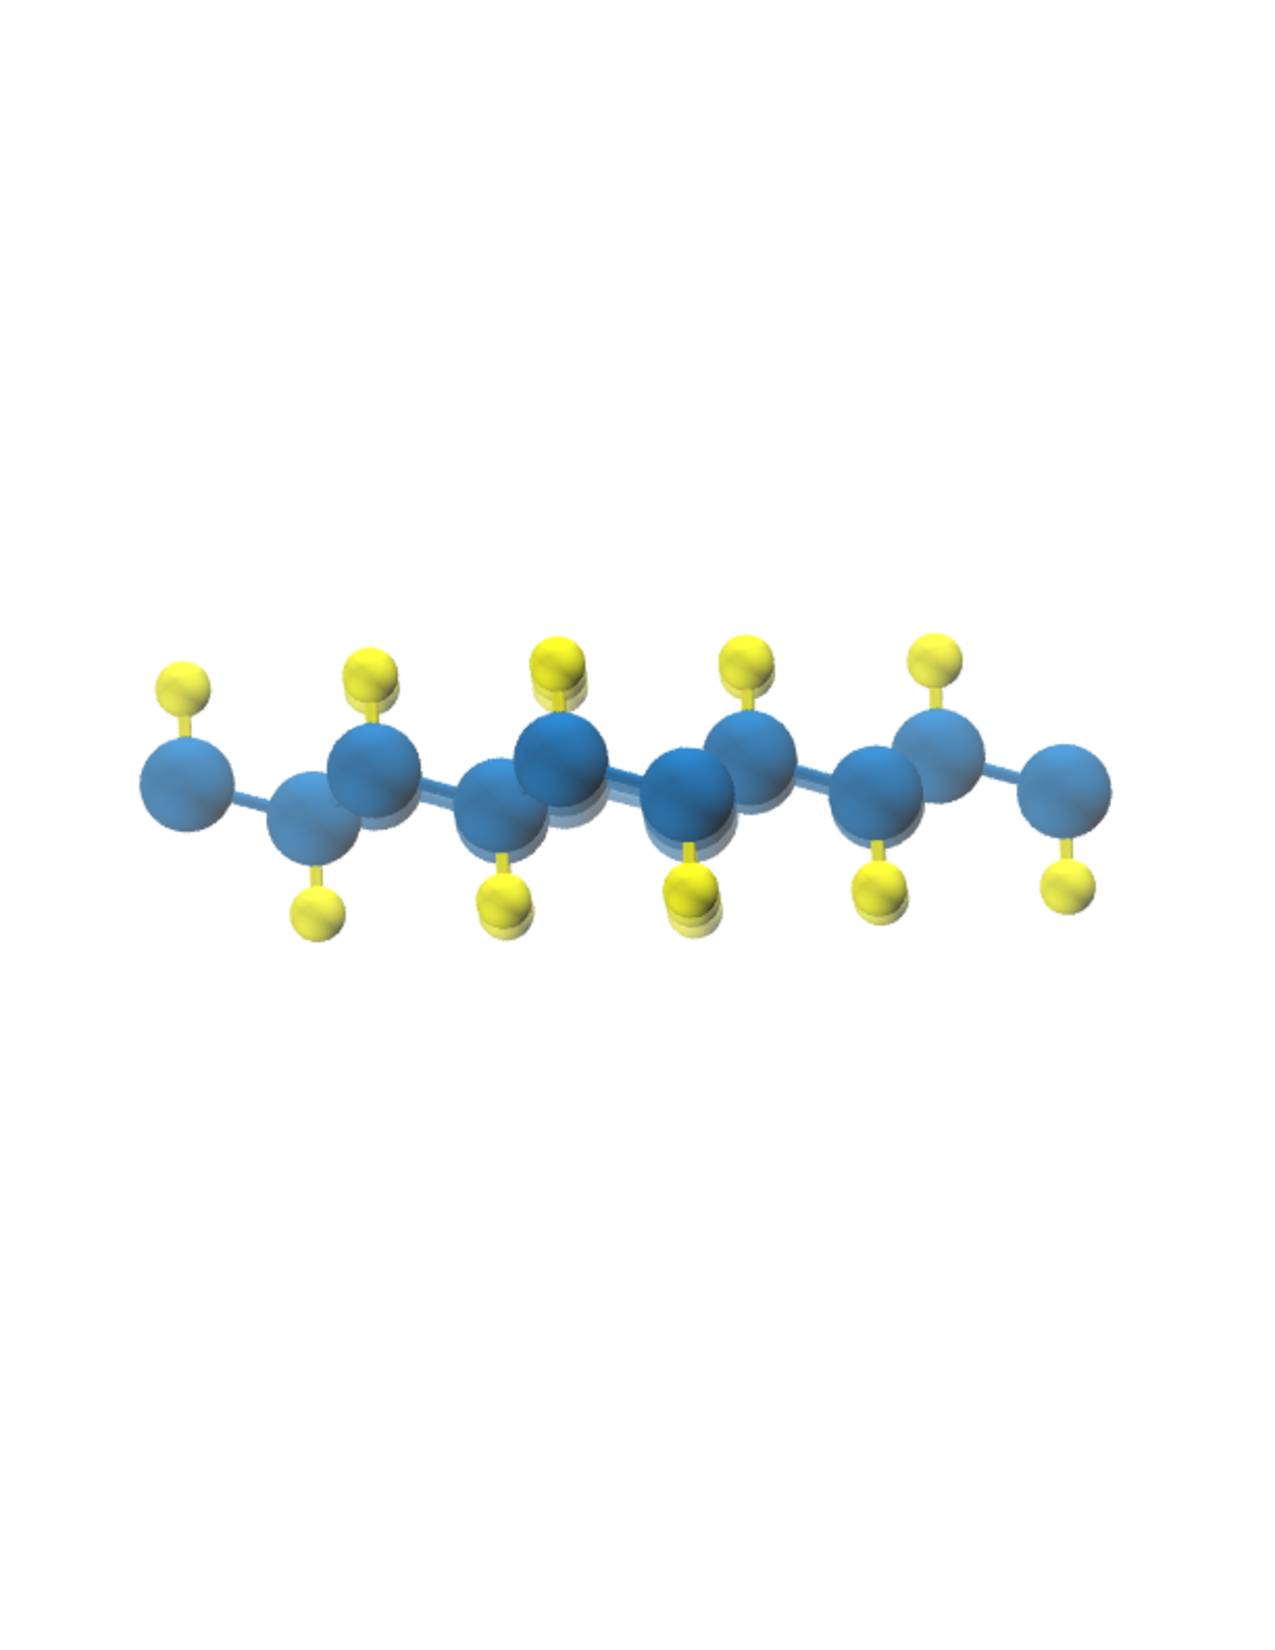
\includegraphics[width=\textwidth]
			{graphane_diagram_cropped}
		\centering \textit{(a)} Side View
	\end{minipage}
	\hfill
	\begin{minipage}[Test 2]{0.475\textwidth}
		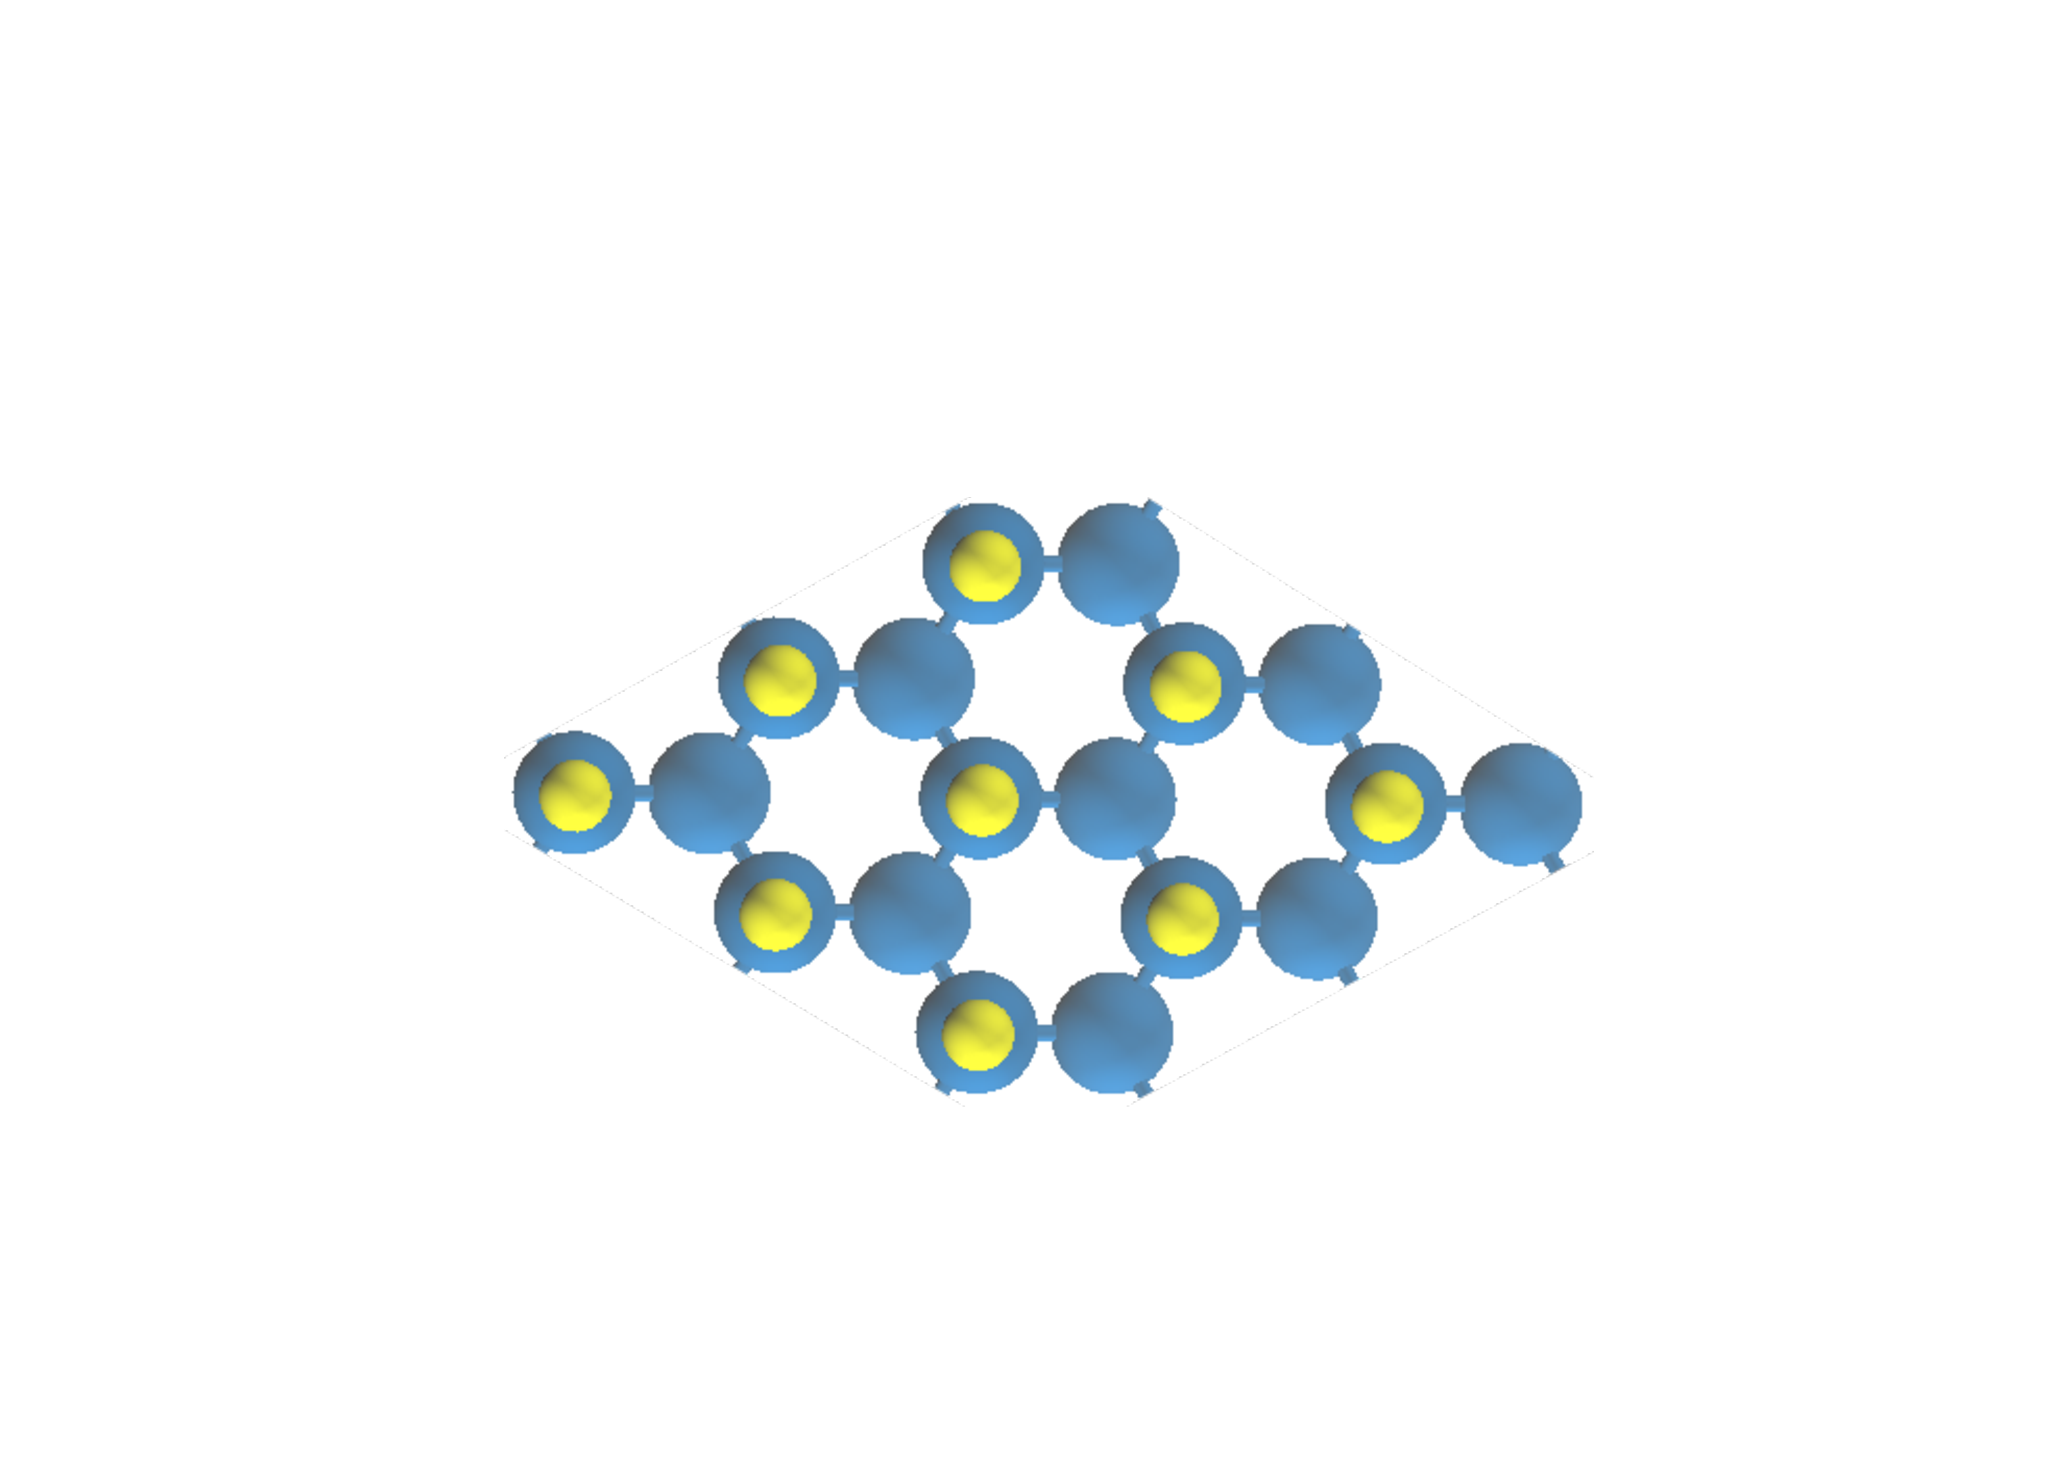
\includegraphics[width=\textwidth]{graphane_diagram_top}	\\
		\centering \textit{(b)} Top View
	\end{minipage}
	\raggedright
	\caption[Diagram of Graphane Structure]{A visual depiction of 
		the graphane structure. Note the alternating above-below 
		scheme and lattice buckling apparent in \textit{(a)}.}
	\label{fig:GraphaneDiagram}
\end{figure}

However, graphane by itself is not very useful for hydrogen storage 
even though it provides a hydrogen atom for every carbon atom in 
the lattice. Graphane is a very stable structure which makes 
extracting the hydrogen atoms an energy consuming task. To break 
the strong, covalent bonds ($\sim 6.56$ eV / atom) that have formed between the carbon and 
hydrogen atoms\cite{SofoChaudhari2007}, we would have to heat the structure---again drawing 
from another energy source---to the point that the energy lost 
balances the energy gained. Even with that fact aside, atomic 
hydrogen (H) is much less useful as a fuel source than molecular 
hydrogen ($\mathrm{H_{2}}$).  We need a structure that binds pre-formed hydrogen molecules and, because of its stability, graphane 
does not.

We can remedy this problem by making a small modification to the 
graphane structure. By replacing some of the hydrogen adatoms with 
metal atoms, we can create a structure that might bind a reasonable 
amount of molecular hydrogen. The buckling induced in the graphene 
monolayer by the hydrogen atoms aids in the binding of these 
metals.

Computational work has already been performed examining calcium and 
lithium as the adatoms with promising results. Hussain \textit{et 
al.} have explored both of these metals and report a hydrogen 
storage capacity of 6 wt. \% for calcium\cite{HussainPathak2012} 
and 12 wt. \% for lithium\cite{HussainDeSarkar2012, 
HussainMaark2012, HussainDeSarkar2014, HussainPathak2011}, both 
with reasonable adsorption energies.

\section{Our Project}
\label{sec:our_project}

In this paper, we also explore computationally the possibility of 
using a graphene monolayer with calcium and hydrogen adatoms as a 
practical solution to the hydrogen storage problem. However, our 
work goes beyond the work that has previously been carried out in 
two ways. 

Firstly, we allow for "vacancies"---carbon sites with no 
corresponding atom in the adsorbant monolayer. With vacancies in 
the structure, the calcium adatoms may have the ability to interact 
with more of the carbon atoms, producing higher binding energies 
between the carbon layer and the adatom layer. Larger spacing 
between the adatoms might also reduce the tendency to cluster, 
allowing for higher concentrations of calcium in the structure and 
hopefully, by extension, increasing the structures's capacity for 
hydrogen storage.

Secondly, we examine structures from a multitude of computational 
unit cell sizes and shapes. This adds a significant degree of 
complexity to structure enumeration, but other members of our group 
have developed methods to speed up the computation. Traditionally, 
only one diamond-shaped unit cell has been studied which greatly 
limits the possible atomic configurations that can be acheived. We 
use the UNiversal CLuster Expansion (UNCLE) code\cite{LerchUNCLE}  
to enumerate many different cell shapes that contain up to the same 
number of atoms as the traditional unit cell (see Figure 
\ref{fig:unit_cells}). By using this type of structure enumeration, 
we hope to discover new structures with promising energetics.

\begin{figure}
	\centering
	\begin{minipage}{0.475\textwidth}
		\centering \textit{(a)} Volume 4 ($2\times2$)
		\includegraphics[width=\textwidth]
			{unit_cell_plots/77}
	\end{minipage}
	\hfill
	\begin{minipage}{0.475\textwidth}
		\centering \textit{(b)} Volume 5 ($1\times5$)
		\includegraphics[width=\textwidth]{unit_cell_plots/96}
	\end{minipage}
	\\ \bigskip
	\begin{minipage}{0.475\textwidth}
		\centering \textit{(c)} Volume 7 ($1\times7$)
		\includegraphics[width=\textwidth]
			{unit_cell_plots/849}
	\end{minipage}
	\hfill
	\begin{minipage}{0.475\textwidth}
		\centering \textit{(d)} Volume 9 ($3\times3$)
		\includegraphics[width=\textwidth]{unit_cell_plots/11130}	\\
	\end{minipage}
	\raggedright
	\caption[Example of Different Unit Cells]{Examples of the 
		different computational unit cells used in structure 
		enumeration. The cells are defined by the periodic black 
		lines in the drawings. The blue circles represent carbon 
		atoms in the graphene lattice. Yellow and red circles 
		represent hydrogen and calcium adatoms respectively. A 
		thick border around an adatom signifies that the atom is 
		below the plane. Note that the structure in \textit{(d)} is 
		a two-dimensional representation of the same structure 
		pictured in Figure \ref{fig:GraphaneDiagram}.}
	\label{fig:unit_cells}
\end{figure}

We begin by briefly summarizing some key concepts and providing 
definitions for important terms. We will outline the computational 
algorithms used for structure enumeration, selection, and 
prioritization. We conclude with a presentation of the results we
obtained. We compare structures with no vacancies against 
structures with vacancies and analyze what we find by searching a 
variety of cell shapes and sizes. We also make mention of several 
directions for future work in the field, many of which are 
currently being explored by our group. 

\chapter{Methods}

\section{Methods Common to Other Groups}
\label{sec:common_methods}

\subsection{Density Functional Theory}

We ran simulations using the Vienna Ab-Initio Simulations Package 
(VASP)\cite{KresseMDLiqMetals, KresseMDGermanium, 
KresseEfficiencyPWBasis, KresseIterativeSchemes} code which peforms 
calculations based on Density Functional Theory (DFT). DFT, as the 
name suggests, uses functionals of electron density to model atoms 
and their interactions (citation). In the simplest of terms, a
\textit{functional} is a function of another function. In other 
words, it is a function that takes in a vector and maps it to a 
scalar. In the case of modeling molecular structure energetics, the 
energy functional is of greatest interest. It takes in the electron 
density function at a given point and returns a scalar energy 
value. To find energetically favorable structures, then, the goal 
is to minimize the energy functional for each 
structure. 

A drawback to DFT is that it is somewhat inaccurate in the 
calculation of weak van Der Waals forces which play a large role in 
the carbon-hydrogen-metal systems being studied (citation). At the 
heart of this problem is the fact that VASP makes use of two 
notable approximations to increase computational speed. In the 
Local Density Approximation (LDA), the energy functional only 
depends on the density at the point where the functional is being 
evaluated. A slightly modified approach called the Generalized 
Gradient Approximation (GGA) is similar except that it also takes 
into account the gradient of the density at the point being 
evaluated. Both of these approximations have been shown to 
inaccurately represent the van Der Waals interactions, with LDA 
overestimating and GGA underestimating.\cite{HussainPathak2012} 
That being said, for simulations with more than just a few atoms, 
these methods are industry standards and the best that we can do.

\subsection{Cluster Expansion}

Cluster Expansion (CE) provides a mathematical model from which we 
can predict the energies of a comprehensive space of structures 
based on the calculated energies of a few structures. CE gets its 
name from the "clusters", or combinations of occupied sites, that 
are summed together to represent a structure. Each cluster has an 
associated weight term which represents energy in this case. 
Clusters and their weights model the interaction between the atoms 
that make up the cluster. Clusters can be defined by a single 
atom (a 1-body cluster) or include any number of atoms in the 
lattice (an \textit{n}-body cluster). As we include more clusters, 
the accuracy of the model increases until, in the limit of 
including all possible structures, it approaches the actual energy 
of the structure. However, we can obtain excellent results even 
with a significant truncation. UNCLE truncates the expansion after 
6-body clusters.

\begin{comment}
Include some sort of explanation of the difference between the 
lattice and the sites where the atoms are located.  Symmetry is 
really what defines the lattice.  For our case, we deal with a 
hexagonal lattice because we only have to rotate the lattice 60 
degrees to obtain an identical lattice.
\end{comment} 

The cluster expansion model is defined by the following equation:		
	\begin{equation} \label{ce_summation}
		E_{\sigma}=\sum_{c}{\Pi_{\sigma c}J_{c}} 
	\end{equation}
where $\sigma$ represents a particular structure and $c$ represents 
a particular cluster. The $E_{\sigma}$ term represents the known 
(calculated) energy of the structure $\sigma$. The $\Pi$ matrix is 
a matrix of correlation values between structures and clusters. The 
rows in the matrix represent structures and the columns represent 
clusters. Finally, the $J_c$ term is an energy "weight" for a given 
cluster. For visualization's sake, it may be easier to understand 
in matrix form.
	\begin{equation} \label{ce_matrix}
		\begin{bmatrix}
			E_1 \\
			E_2 \\
			\vdots \\
			E_n
		\end{bmatrix}
		=
		\begin{bmatrix}
			\Pi_{11} & \Pi_{12} & \cdots & \Pi_{1m} \\
			\Pi_{21} & \Pi_{22} & \cdots & \Pi_{2m} \\
			\vdots   & \vdots   & \ddots & \vdots \\
			\Pi_{n1} & \Pi_{n2} & \cdots & \Pi_{nm}
		\end{bmatrix}
		\begin{bmatrix}
			J_1 \\
			J_2 \\
			\vdots \\
			J_m
		\end{bmatrix}
	\end{equation}
In other words, the energy of a given structure is simply the sum 
of the properly weighted terms in the row of the $\Pi$ matrix that 
represents the structure. If the $\Pi$ matrix were square, we could 
simply invert the matrix and multiply to find the weights. However, 
the number of clusters and the number of structures do not have to 
be (and rarely are) equivalent. This generally results in a an 
underdetermined system for our purposes and more complex linear 
algebra techniques are required to solve it. Fortunately, Nelson 
\textit{et al.} have developed Bayesian Compressed Sensing methods 
to solve this system efficiently.\cite{NelsonCE}

Once the weights are found, the multiplication on the right side of 
Eq. \ref{ce_summation} predicts the energy for any structure in the 
space.

\section{Enumeration of Structures}

We use the UNCLE code to perform enumeration of all possible 
symmetrically inequivalent structures in a given space. UNCLE 
performs a solely mathematical enumeration based on the shape of 
the lattice and the adatom options at each lattice site. This type 
of enumeration will inevitably produce structures that could not 
possibly exist in nature due to the size of the adatoms. For 
example, because the atomic radius of a calcium atom is large ($
\sim$1.74 \AA) and carbon-carbon bond lengths in the graphene 
lattice are not ($\sim$1.42 \AA), we cannot place two calcium atoms 
adjacent to one another. Pairs of atoms that cannot be placed next 
to each other are termed \textit{forbidden pairs}. We do not want 
to waste time in the search running "forbidden" structures through 
VASP calculations so, to this end, other members of our group have 
added functionality to exclude them from the enumeration (reference 
Joseph's paper). 

Our enumeration, however, is left somewhat incomplete. From sets of 
structures that are rotationally or translationally equivalent 
(like 10 and 01) we only keep one. We then use \textit{tiles} of 
the remaining symmetrically inequivalent structures to build up our 
computational unit cells. Because we form the tiles after 
elimination by symmetry, some tiles are not available for use and, 
thus, some structures are left out of the enumeration. This does 
have a positive consequence, though, in that we can perform higher 
volume enumerations and explore higher volume structures in our 
search than we could otherwise.

\section{Search for Favorable Structures}

The main portion of my work in the group dealt with creating, 
coding, and automating the iterative process of searching the space 
of possible structures. The basic algorithm can be seen in Figure 
\ref{fig:ProcessDiagram}. It starts by selecting a set of what are 
called independently and identically distributed (IID) structures 
to use as initial input to the iteration loop. IID means that the 
initial set will include structures that are as different as 
possible from one another.

\begin{figure}
    \centerline{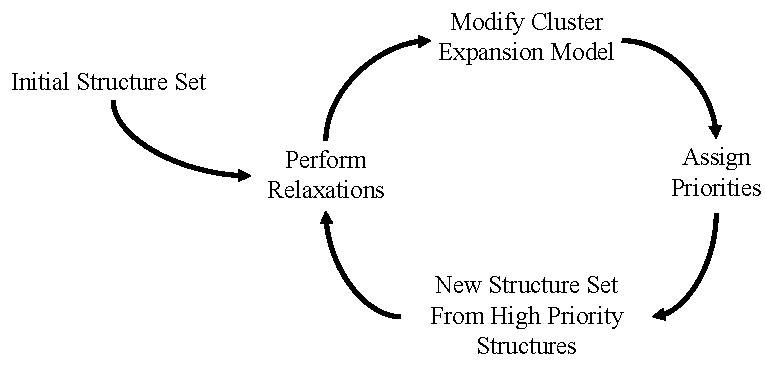
\includegraphics{Erik_Swenson_Schematic}}
    \caption[Search Process Schematic]{A high level map of the 
    		iteration process. We start with a randomly selected set of 
    		structures. We run the structures through atomic and 
    		electronic relaxation routines and use that data to create 
    		a predictive model for all possible structures. We then 
    		assign each structure a priority and choose a set of 
    		highest priority to run back through the loop.}
	\label{fig:ProcessDiagram}
\end{figure}

Our new code takes the IID structure set and extracts the important 
information into a format that VASP can work with. VASP iteratively 
makes slight adjustments to the positions of the ions and the 
electrons in order to minimize the energy of the structure in a 
process called \textit{relaxation}. 

Once VASP has found the energy-minimized configuration for each 
structure, we create a CE model based on the results from this 
initial structure set. The model predicts the energy of all the 
structures in the space. (Initially, this model is not very 
accurate, but as we add more structures to the model each 
iteration, the accuracy increases substantially.) We prioritize the 
structures according to a decaying exponential scale. Energetically 
favorable (low energy) structures are given high priority while 
high energy structures are given a much lower priority.

We then select a new set of the highest priority structures from 
the pool of structures that have not been run through VASP 
calculations and the loop begins again. It should be noted that, 
because we choose new structures at the end of each iteration based 
on their priority, the energy-predictive model we refine may not be 
very accurate for higher energy structures. This is not an issue 
since high energy structures are of no practical interest to us 
anyway. 

\chapter{Results}

\section{Energy Metrics}

When analyzing the results of our energy calculations, the most 
intuitive metric we use to summarize a structure's energy is 
formation energy. Formation energy (FE) is defined as the average 
energy per adatom required to pull the adatoms out of reference 
structures and bind them to the graphene layer. For hydrogen, we 
use a hydrogen molecule as the reference structure and for calcium, 
the reference structure is a hexagonal monolayer of calcium atoms 
bound together. Mathematically,
	\begin{equation} \label{form_E}
		\mathrm{FE}_{struct} = \frac{\mathrm{E}_{struct} - 
			\left(\mathrm{E}_{graphene} + \sum\limits_{i}
			{\mathrm{n}_{i}\mathrm{E}_{i}^{ref}}\right)}
			{\sum\limits_{i}{\mathrm{n}_{i}}}
	\end{equation}
where $\mathrm{E}_{struct}$ is the energy value of that structure 
directly from the calculations, $\mathrm{E}_{graphene}$ is the 
calculated reference energy of graphene, and the summation term 
gives the number of each type of adatom multiplied by its 
corresponding reference energy. The denominator simply tells us to 
divide by the number of adatoms.

Another important metric used in our analysis is planar binding 
energy (PBE) which, in the most simple terms, tells us how much 
energy is required to separate the adatom layers from the carbon 
monolayer far enough that the interaction between the layers is 
negligible. Structures with positive or weakly negative PBE are 
essentially already separated into layers. Mathematically,
	\begin{equation} \label{pbE}
		\mathrm{PBE}_{struct} = \mathrm{E}_{struct} - 
			\left(\mathrm{E}_{graphene} + 
			\mathrm{E}_{adatoms}\right) 
	\end{equation}
where $\mathrm{E}_{struct}$ and $\mathrm{E}_{graphene}$ carry the 
same meaning as in FE and $\mathrm{E}_{adatoms}$ represents the 
total energy of the adatom layers with the carbon atoms removed.

Planar binding energy should not be confused with the standard 
binding energy (BE) of individual calcium atoms to the 
carbon-hydrogen structure. BE tells us how much energy it would
take to pull the calcium atoms far enough away that they have no 
interaction with the rest of the structure. We will use BE as a 
comparison metric to other structures in the literature. 

Our goal is to find structures that exhibit a strong FE as well as 
a strong PBE. To this end, we have defined a fourth, non-physical 
quantity called sorting energy (SE) which is defined as 
	\begin{equation} \label{inter_E}
		\mathrm{SE}_{struct} = 
			max\left(\mathrm{FE}_{struct}, 
			\mathrm{PBE}_{struct}\right)	\quad.
	\end{equation}
When we sort the structures according to their SE, we can easily 
find those that have strong FE as well as PBE.

Figure \ref{fig:FEvsPBE} shows a plot of PBE vs. FE for binary 
double-sided structures. We can see that the region of interest 
representing structures that simultaneously boast low FE and PBE is 
basically empty. There are two tails of structures that skirt this 
region. The tail extending into the low FE region is mostly made up 
of structures that exhibit calcium stacking (discussed in the next 
section) and the tail extending into the low PBE region is mostly 
made up of "graphane-like" structures that contain no calcium at 
all. Neither of these are desirable characteristics for hydrogen 
storage applications and, thus, our focus will be on the structures 
that make some compromise between the two.

\begin{figure}
	\centering
	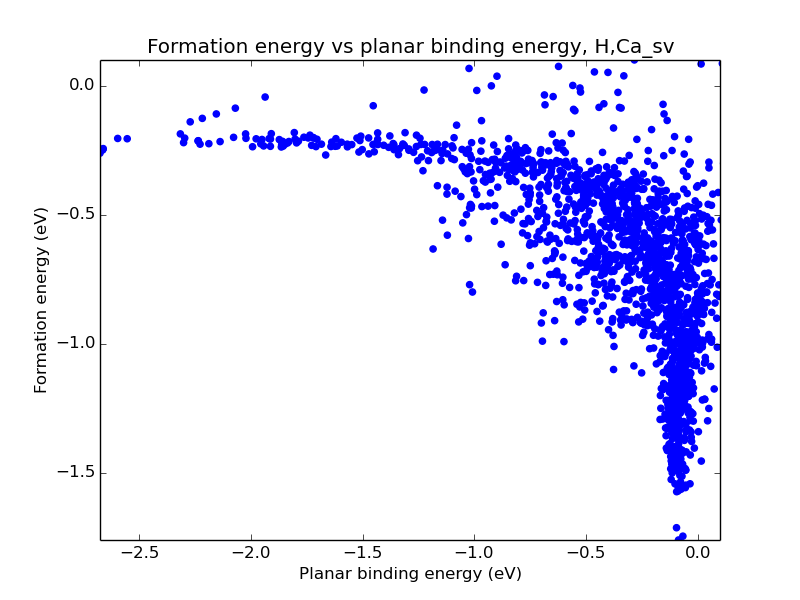
\includegraphics[width=0.6\textwidth]			
		{bin_both_FEvsplanarBE_1.png}
	\caption[Formation Energy vs. Planar Binding Energy]{A plot of 
		formation energy vs. planar binding energy for binary 
		double-sided structures. Each blue dot represents a 
		particular structure. The empty region in the lower left 
		corner of the graph indicates that there is some sort of 
		competition between the two types of energy.}
	\label{fig:FEvsPBE}
\end{figure}

\section{Single-Sided Bonding}

In the single-sided case, we find stable, desirable structures with up to $22.2~\%$ calcium concentration. Figure \ref{bin_top_convex_hull} shows plots of formation energy vs. hydrogen concentration for binary single-sided structures. The red "tie lines" drawn in Figure \ref{bin_top_convex_hull} \textit{(a)} define the \textit{convex hull} of this set of structures. In thermal equilibrium, any structure that has formed will separate into sections that look like the structures on the convex hull. However, at this stage, we do not know anything about how long it will take to reach thermal equilibrium. A structure may not be the lowest energy structure at its concentration, but if the barriers to other lower energy states are high, it may take an impractically long time to reach the lowest energy state. These structures are called \textit{metastable} structures. This makes it difficult to eliminate the possibility of using any structure with weaker energy as hydrogen a storage mechanism, but we will focus on the structures with the strongest energies at each concentrations because they are the most likely to occur in nature.

\begin{figure}
	\centering
	\begin{minipage}{0.49\textwidth}
		\centering
		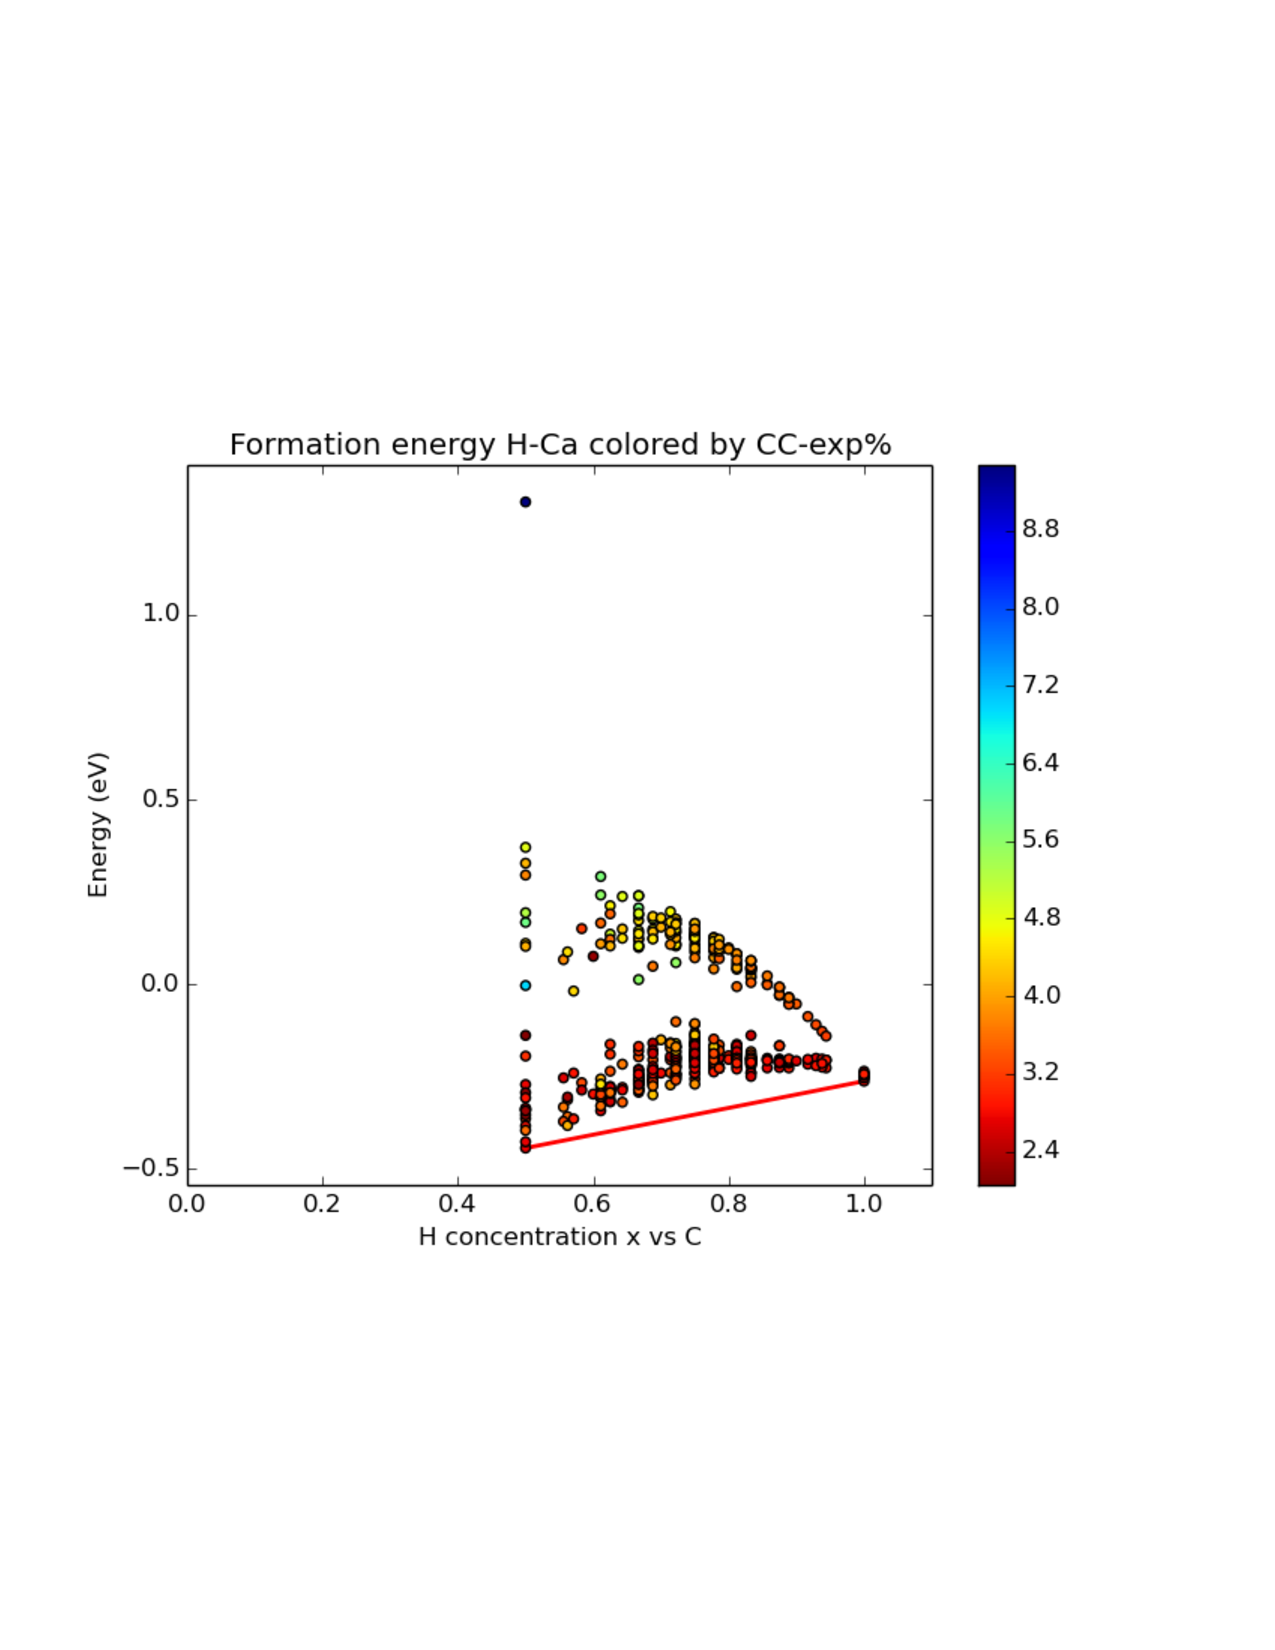
\includegraphics[width=\textwidth]
			{bin_top_FE_CC-exp(atoms0-1)_1} \\
		\textit{(a)}	
	\end{minipage}
	\hfill
	\begin{minipage}{0.49\textwidth}
		\centering
		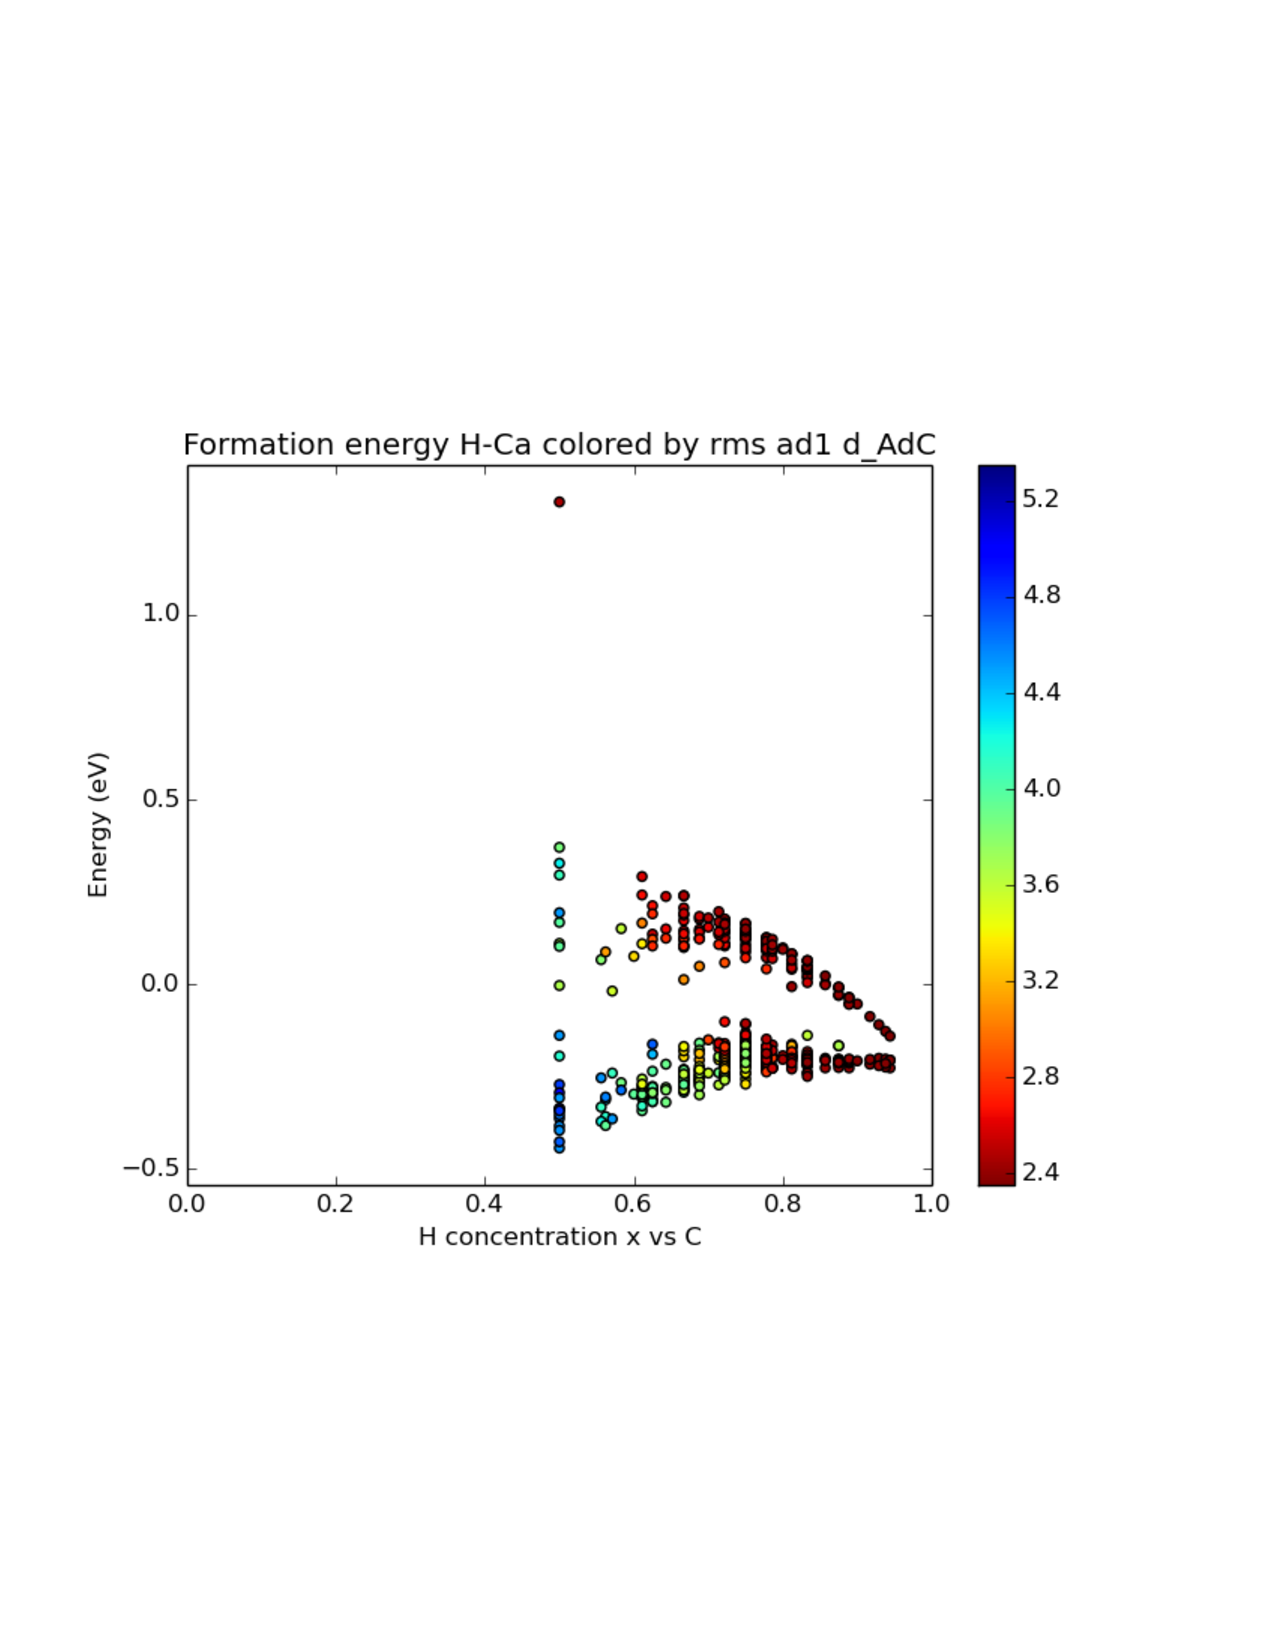
\includegraphics[width=\textwidth]
			{bin_top_FE_rms_ad1_d_AdC(atoms0-1)_1} \\
		\textit{(b)}	
	\end{minipage}
	\caption[Binary Single-Sided Search Data]{Plots of formation 
		energy vs. hydrogen concentration in binary single-sided 
		structures. The coloring of the dots in part \textit{(a)} 
		represents the expansion percentage of the carbon lattice 
		as a result of adding the hydrogen and calcium. The red 
		"tie lines" represent the convex hull: the naturally 
		occurring structures in thermal equilibrium. The coloring 
		of the dots in part \textit{(b)} represents the average 
		distance in angstroms of the calcium atoms from the plane 
		of carbon atoms. "Stacked" structures have a much higher 
		average calcium-carbon distance.}
	\label{bin_top_convex_hull}
\end{figure}

At concentrations greater than $22.2~\%$, the lowest energy structures are less desirable due to "stacking" of calcium atoms perpendicular to the carbon monolayer rather than binding directly to the monolayer. Calcium stacking causes two main problems. Firstly, the stacked calcium atoms create strong bonds with each other, reducing the ability to bind $\mathrm{H_{2}}$ to the structure. As the calcium atoms bond together, they build up and away from the plane of carbon atoms, making the structure much less space-efficient. The coloring of the dots in Figure \ref{bin_top_convex_hull} \textit{(b)} indicates the average distance of the calcium atoms from the carbon monolayer. We can see that, above $22.2~\%$ calcium concentration, the average distance from the plane begins to increase due to calcium stacking. Secondly, the buildup of calcium layers adds extra weight to the structure. We want to create structures that are both space-efficient and lightweight and, therefore, we will discard any stacked structures from our analysis. An visual example of the stacking problem is shown in Figure \ref{clustering_example}.

\begin{figure}[b]
	\centering
	\begin{minipage}{0.45\textwidth}
		\centering
		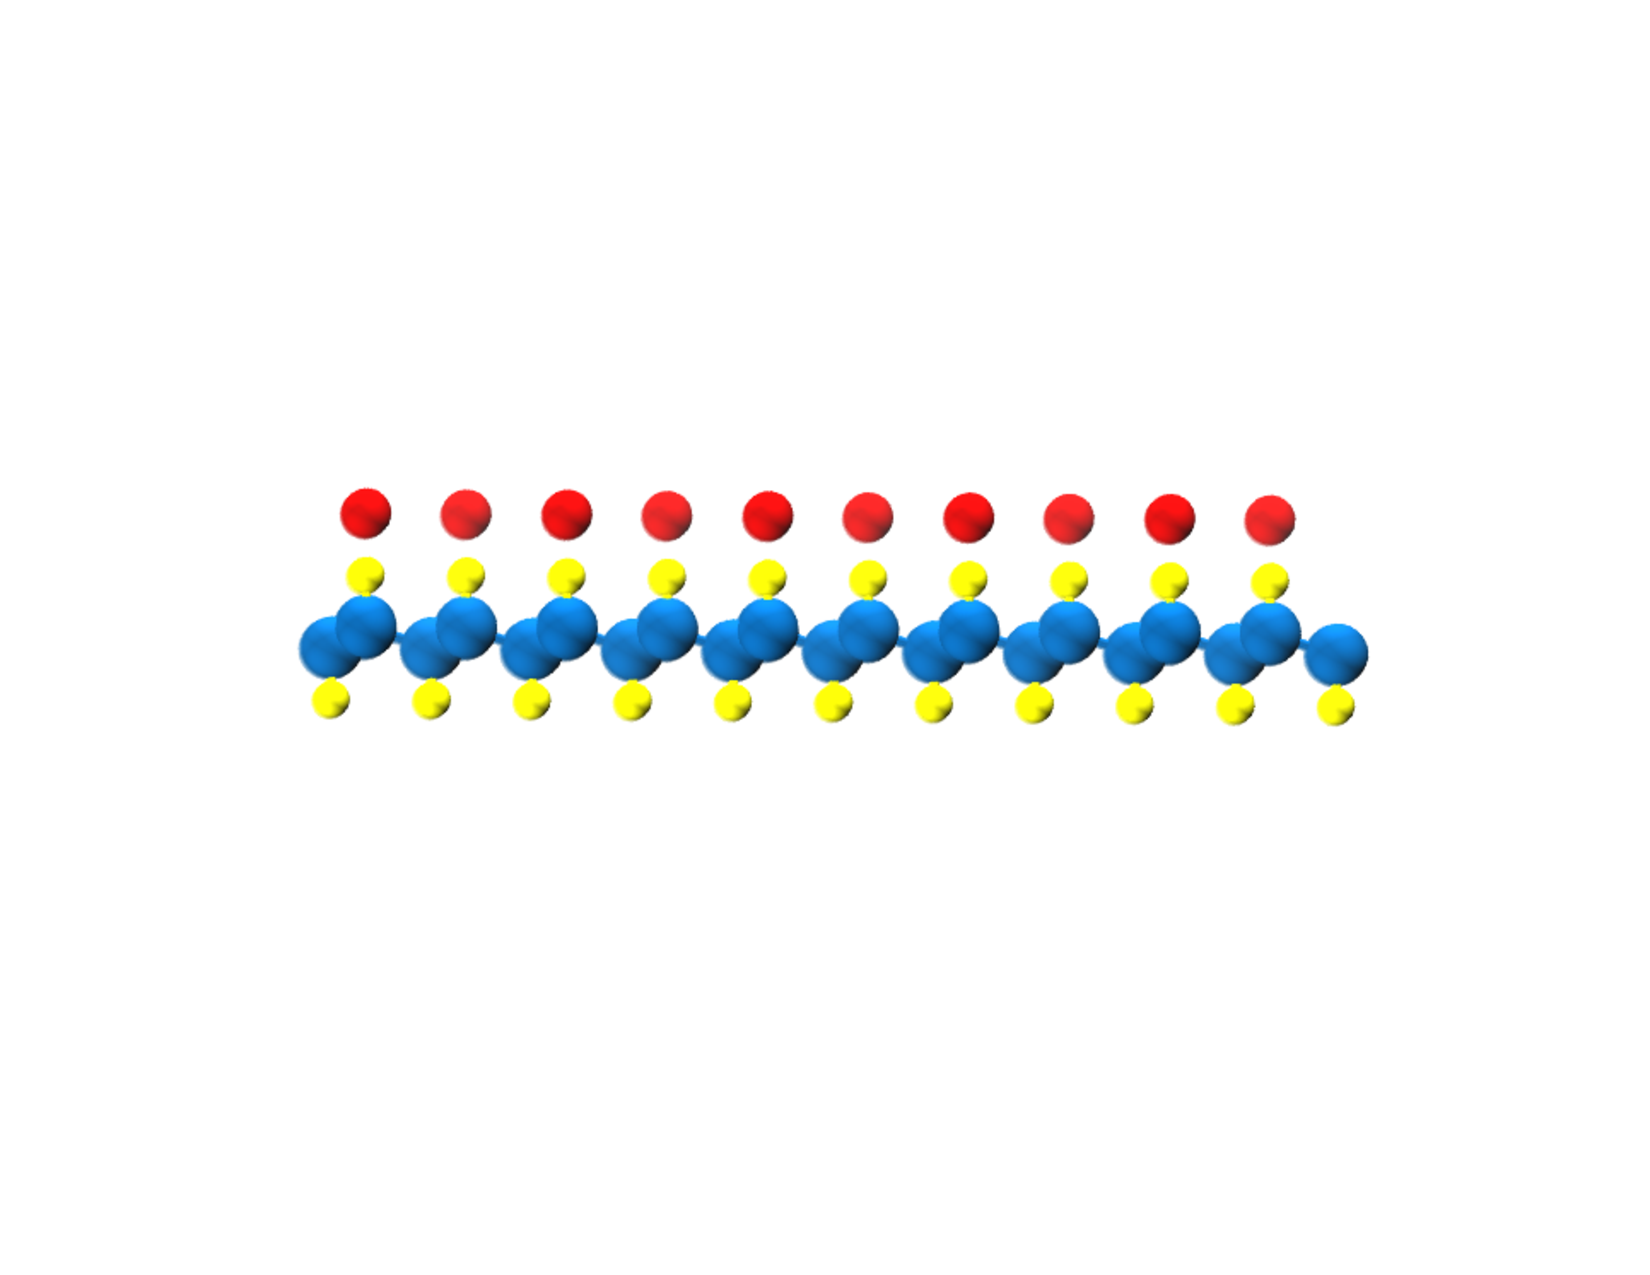
\includegraphics[width=\textwidth]{non_clustering}
		No stacking	
	\end{minipage}
	\hfill
	\begin{minipage}{0.45\textwidth}
		\centering
		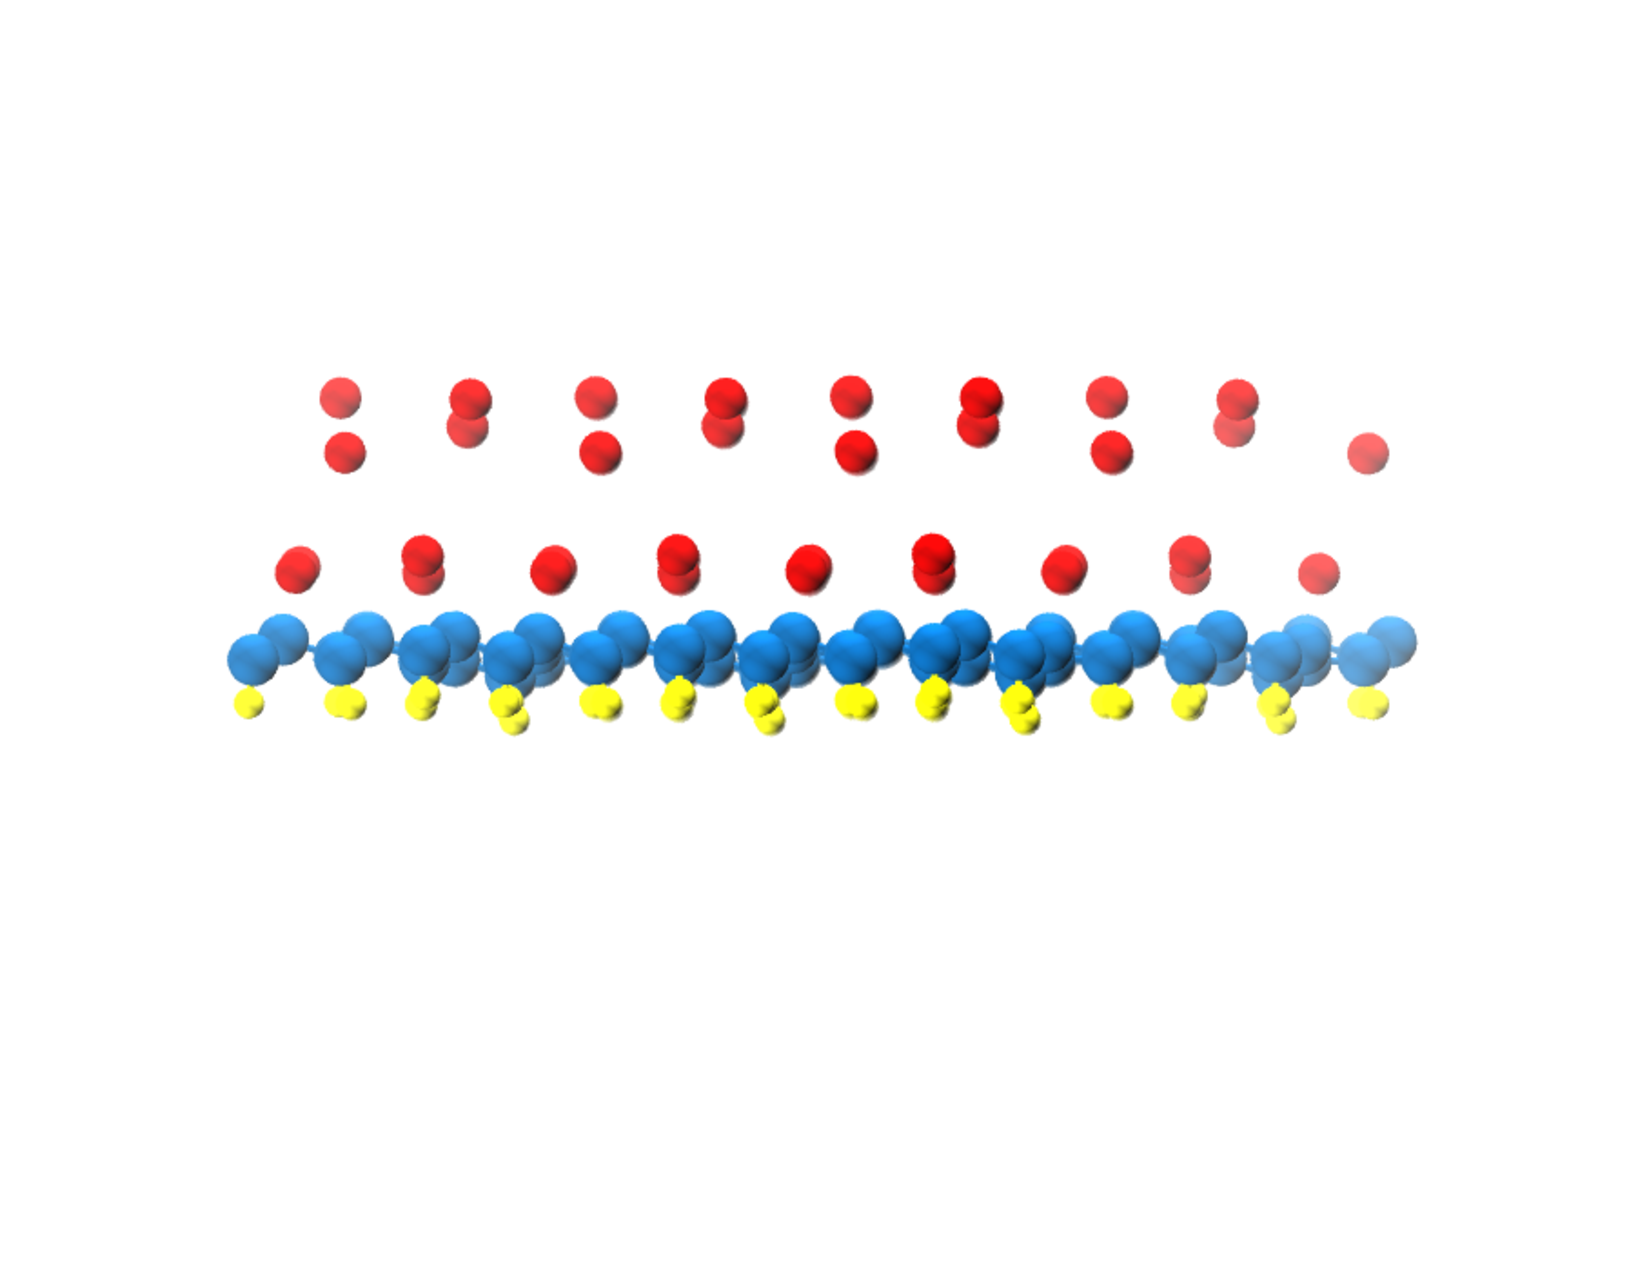
\includegraphics[width=\textwidth]{clustering_example}
		Stacking
	\end{minipage}
	\caption[Example of Calcium Stacking]{An example of calcium 
		stacking. Pictured on the left is the side view of a 
		structure where calcium atoms (red) and hydrogen atoms 
		(yellow) are bound directly to the carbon monolayer (blue). 
		On the right is the side view of a structure that exhibitis 
		calcium stacking. Calcium atoms bond with each other rather 
		than the carbon monolayer and build up perpendicular to the 
		plane, wasting valuable space in the structure.}
	\label{clustering_example}
\end{figure}

The most stable binary single-sided structure at 22.2\% calcium concentration is pictured in Figure \ref{bin_top_222_struct} with $\mathrm{FE} = -0.229~eV$ and $\mathrm{PBE} = -1.19~eV$. There are, of course, other structures at different concentrations with stronger energies, but we want to find those with the highest calcium concentrations and without calcium stacking. This structure fits both of those criteria.

\begin{figure}
	\centering
	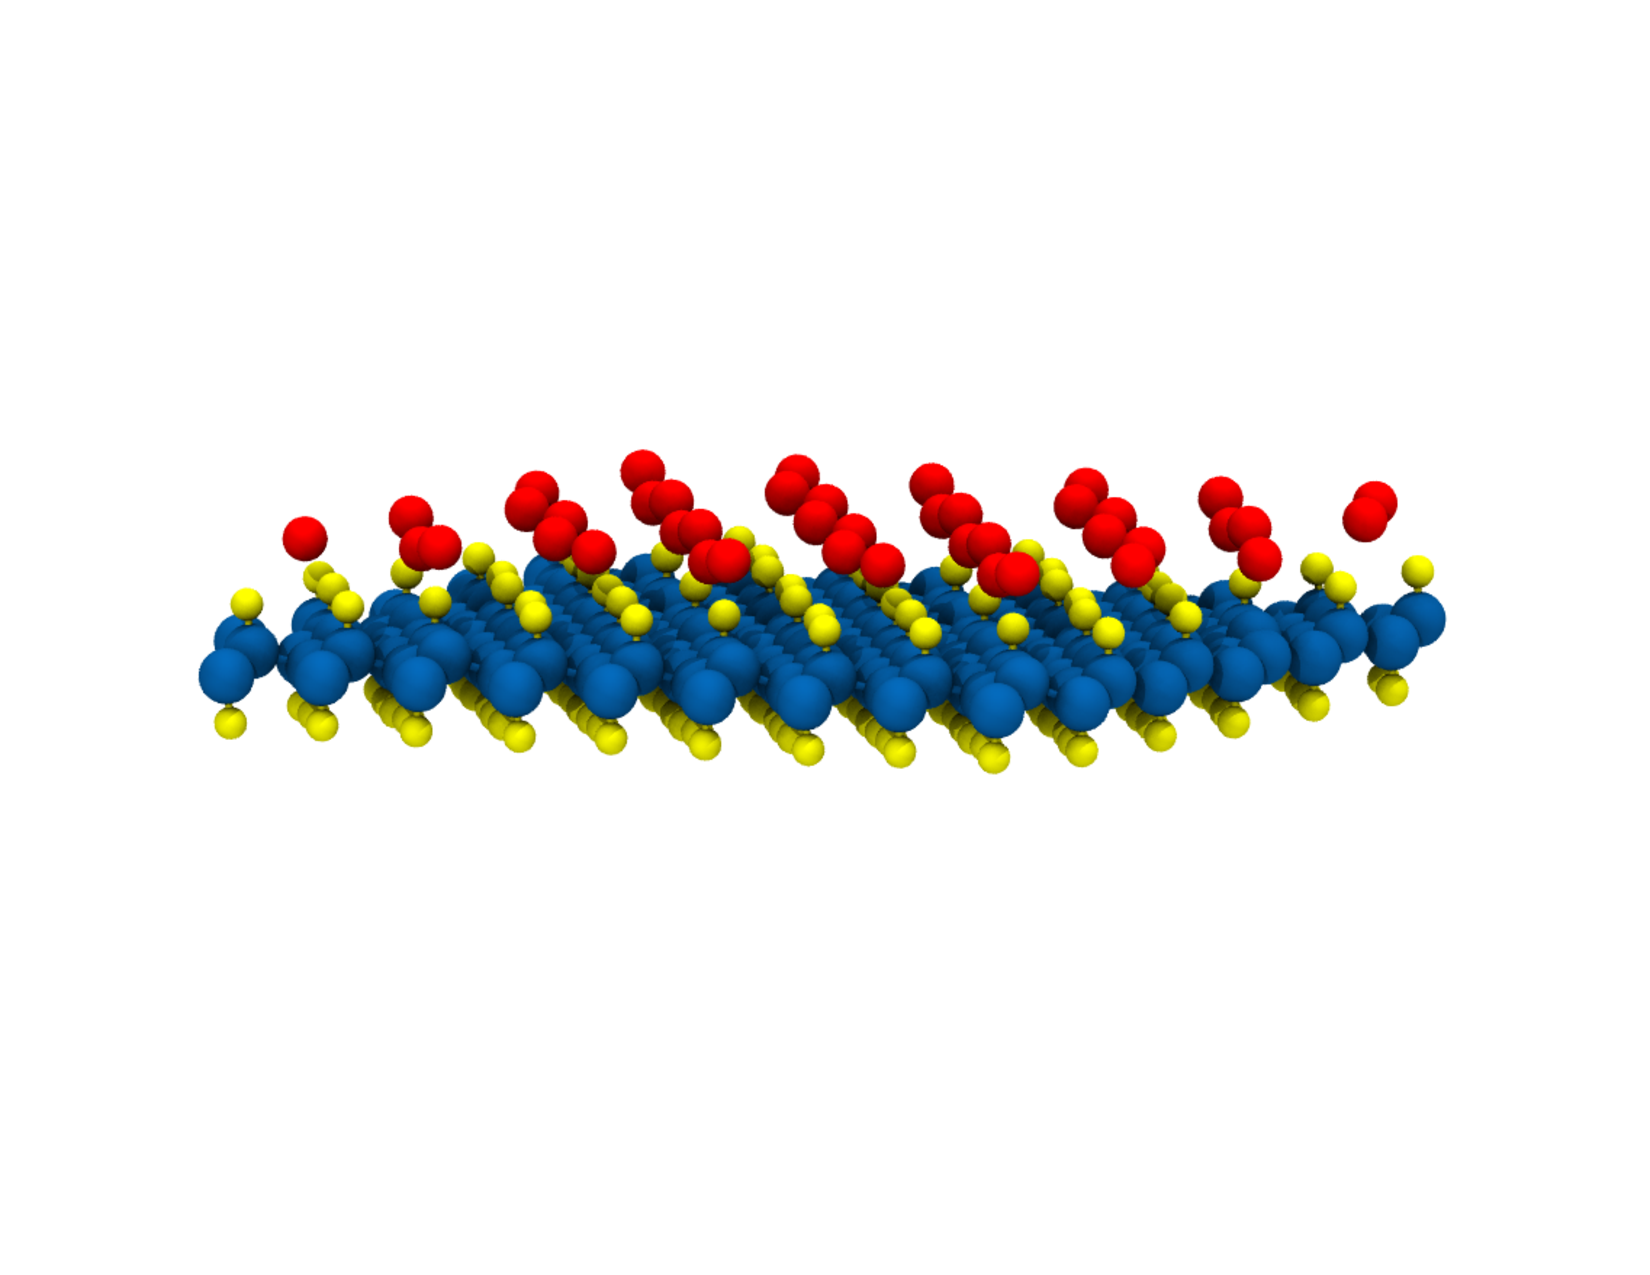
\includegraphics[width=0.6\textwidth]{bin_top_222_struct}
	\caption[Stable Binary Single-Sided Structure]{A rendering of 
		the most stable binary single-sided structure at 22.2\% 
		calcium concentration without calcium stacking.}
	\label{bin_top_222_struct}
\end{figure}

\subsection{Estimating Error in the Energy Calculations}

If we examine the formation energies closely, we can come up with 
an estimate of the error in the energy calculations. A pure 
graphane structure (100\% hydrogen concentration) can be 
represented with any shape or size of computational unit cell, 
however, in the energy calculations, we should see the same result 
for each graphane structure regardless of cell shape or size. 
Looking at the plot of formation energy for single-sided structures 
shown in Figure \ref{error_estimate}, it is easy to see that there 
is some slight variation in the graphane calculations. Therefore, 
we cannot expect the error on any of the energy calculations to be 
smaller than that spread. The spread in the graphane energy 
calulations is $30~meV$ for FE and $22~meV$ for PBE. These error 
estimates should be applied to all energy calculations presented in 
this paper.

\begin{figure}
	\centering
	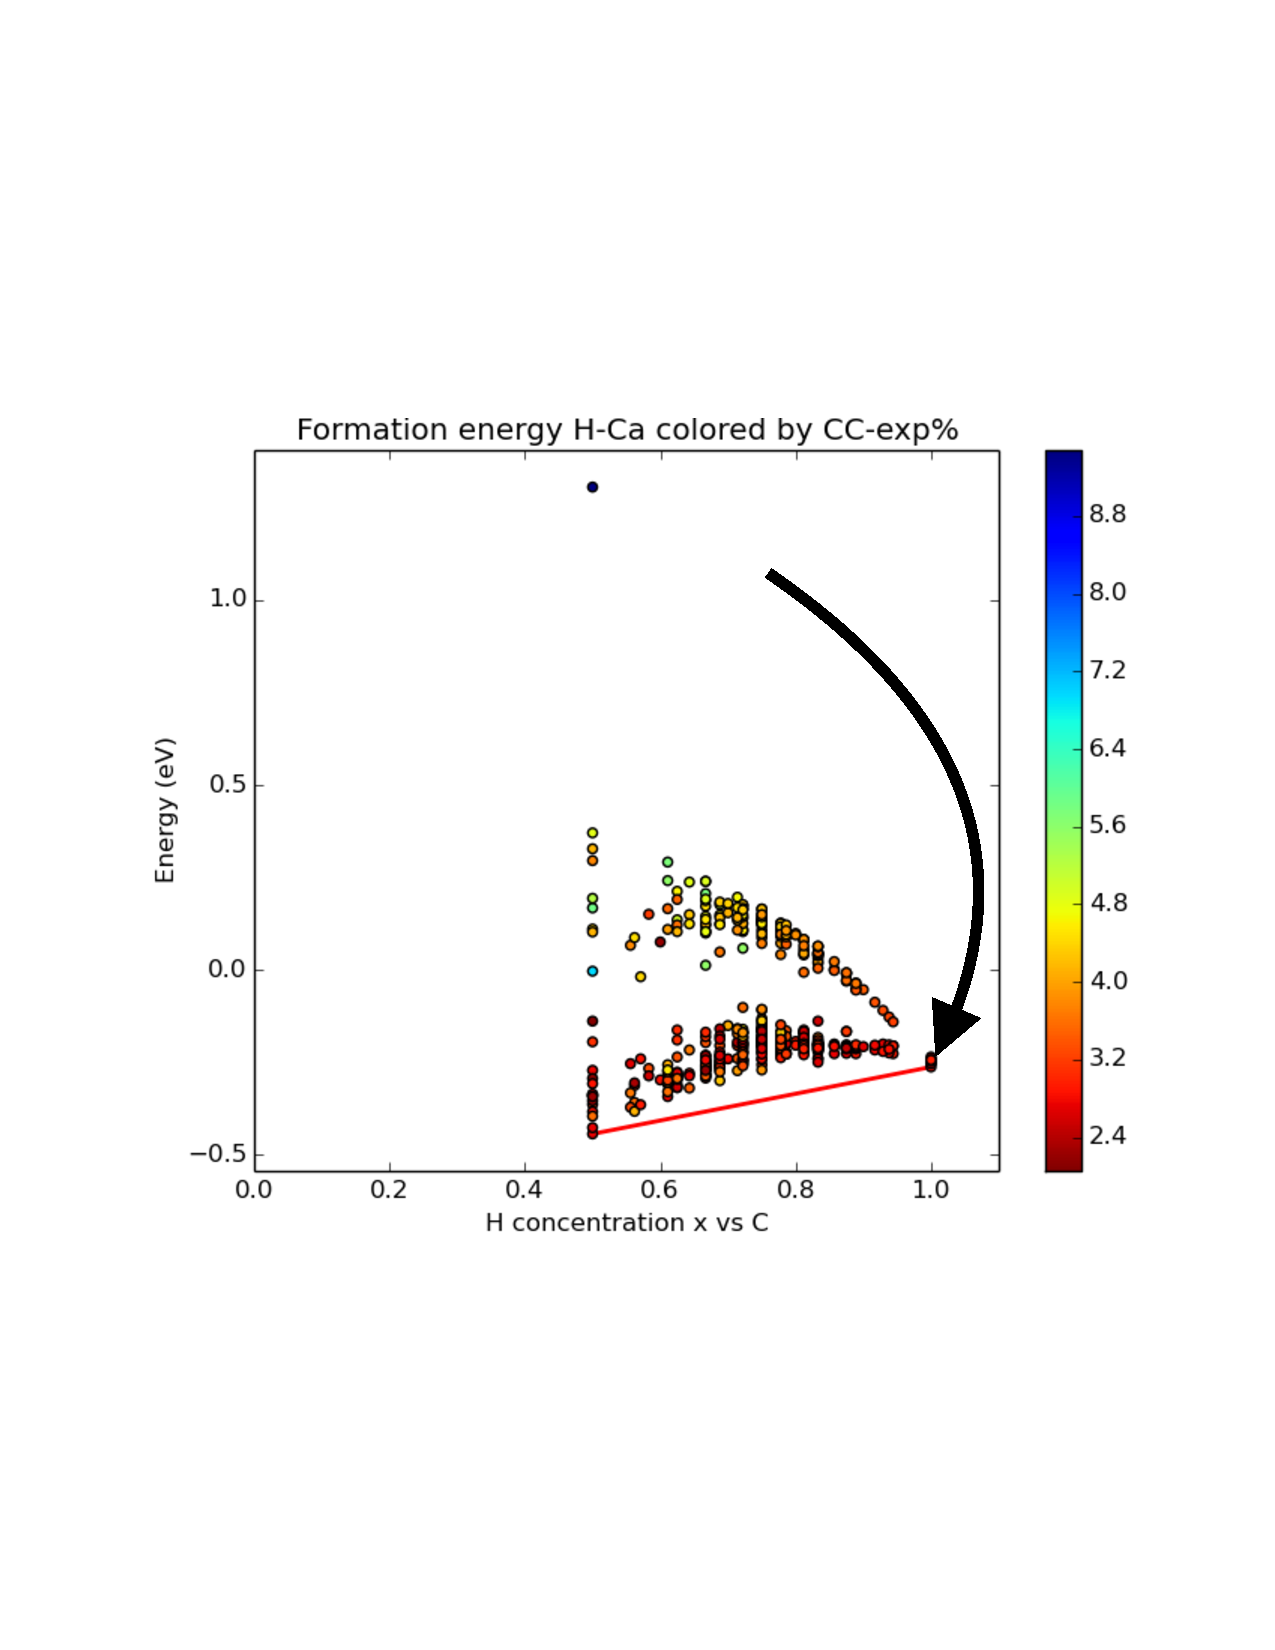
\includegraphics[width=0.6\textwidth]			
		{bin_top_FE_CC-exp(atoms0-1)_1_arrow}
	\caption[Error Estimate From Graphane Calculations]{A plot of 
		formation energy vs. hydrogen concentration with coloring 
		representing the expansion percentage of the carbon lattice 
		(also shown in Figure \ref{bin_top_convex_hull} 
		\textit{(a)}). The slight spread in the graphane energy 
		calculations (indicated by the arrow) gives us an error 
		estimate for all our energy calculations. The spread in 
		formation energy is $30~meV$. }
	\label{error_estimate}
\end{figure}

\section{Double-Sided Bonding}

After analyzing the results from the single-sided search, it is reasonable to expect that structures with high calcium concentrations will likely exhibit stacking. Our hope, though, is specifically to find structures with high calcium concentrations in order to bind higher concentrations of $\mathrm{H_{2}}$ molecules later. Double-sided bonding results in a significant increase in the concentration of calcium atoms that can be acheived without stacking. We conclude that any binary double-sided structure with more than a $30~\%$ calcium concentration will exhibit stacking. We, therefore, limit our analysis to structures under that concentration.

The most stable structure with the $30~\%$ calcium concentration that we found is shown in Figure \ref{bin_both_30_struct}, with $\mathrm{FE} = -327~meV$ and $\mathrm{PBE} = -694~meV$. These energies are much larger than thermal fluctuations ($\sim~20~meV$) indicating that, according to energetics at least, the structure could theoretically exist in nature.

Thermodynamics, on the other hand, suggests that the structure would not occur naturally. The red tie line drawn in Figure \ref{bin_both_convex_hull} \textit{(a)} is called a convex hull. According to thermodynamics, only structures that lie on the convex hull will exist in nature. 

The same structures are plotted in Figure \ref{bin_both_convex_hull} \textit{(b)}, but colored according to the rms distance of the calcium atoms to their nearest neighboring carbon atoms. Stacked structures contain layers of calcium atoms that are much further away from the carbon atoms and, hence, will have a much larger average distance. From this plot, we can see that most of the structures on or even near the convex hull are stacked structures---with the exception of graphane, of course---meaning that, if we allow calcium to be part of the structures, we will probably only be able to produce stacked structures.

\begin{figure}
	\centering
	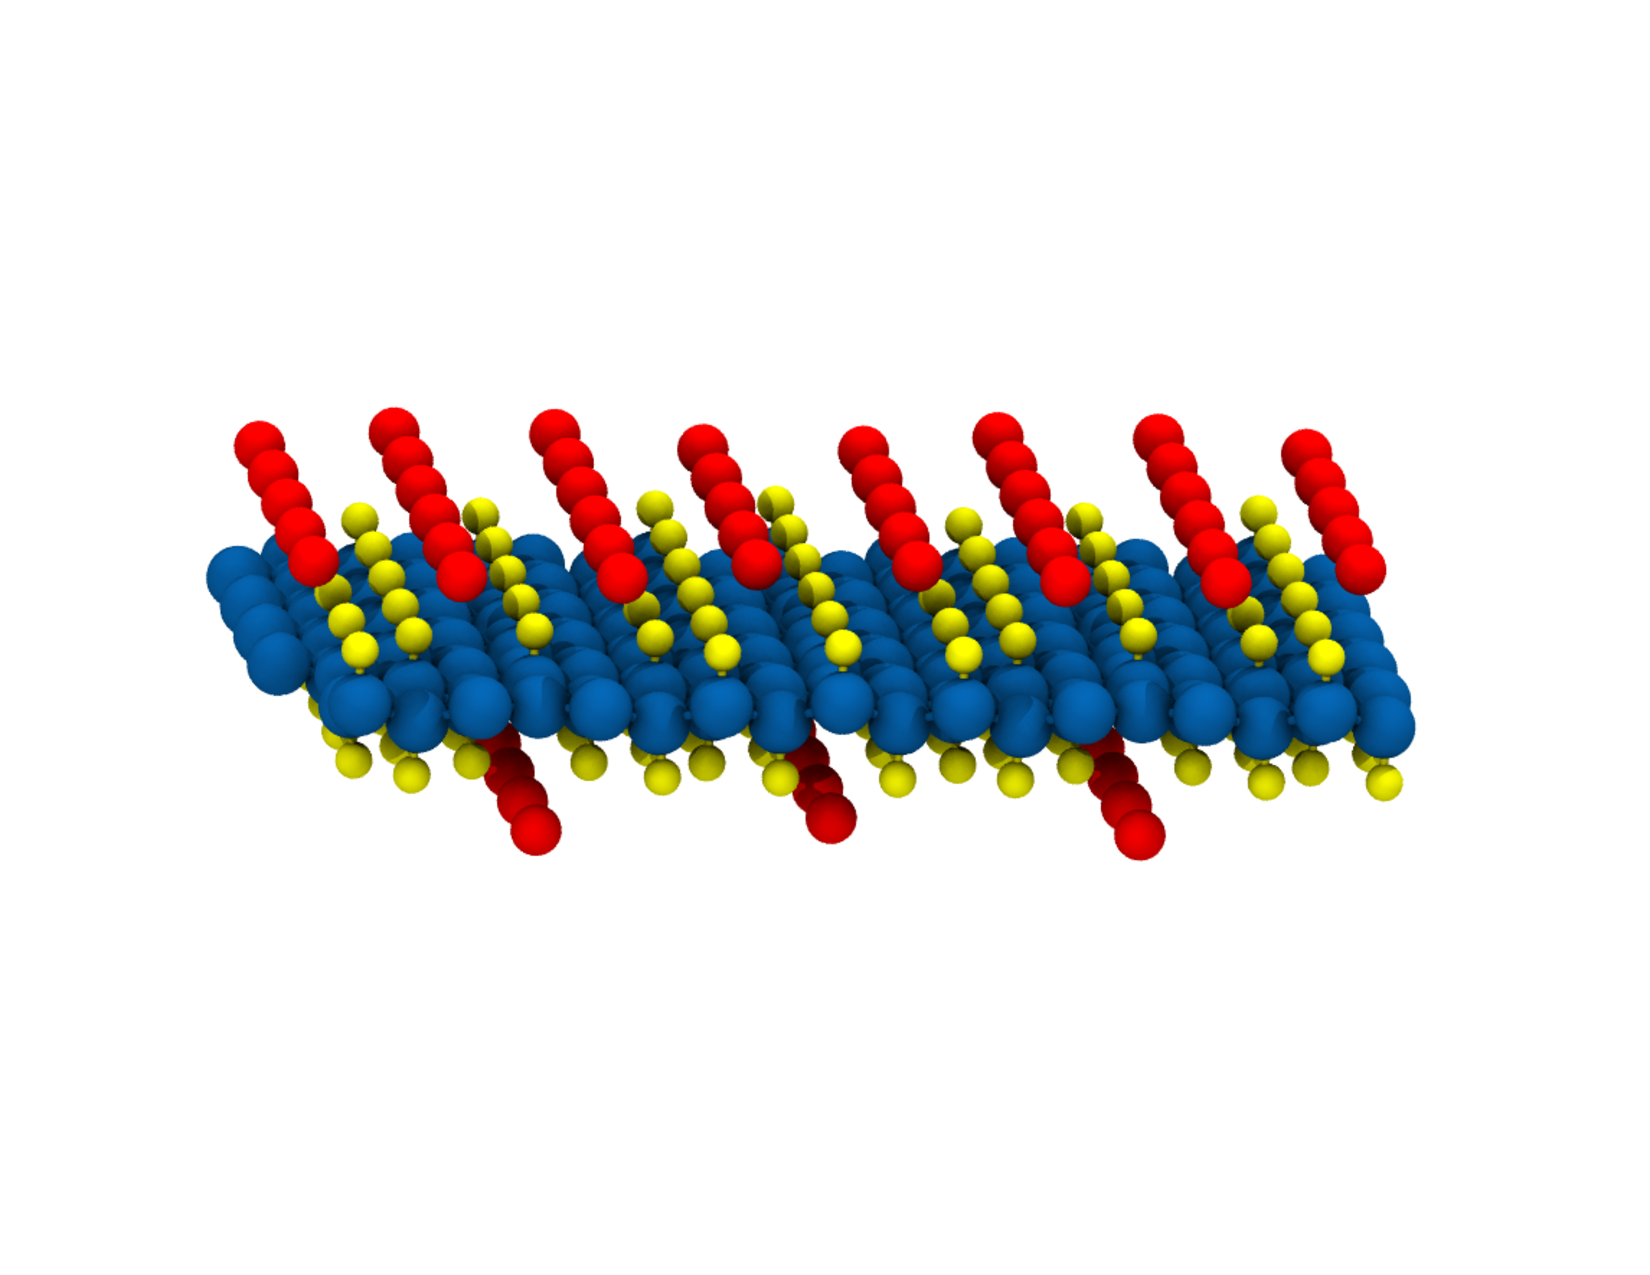
\includegraphics[width=0.6\textwidth]{bin_both_300_struct}
	\caption[Stable Binary Double-Sided Structure]{The binary 
		double-sided structure with the highest concentration of 
		calcium atoms ($30~\%$) that did not suffer from calcium 
		stacking. Again, carbon atoms are blue, calcium atoms are 
		red, and hydrogen atoms are yellow.}
	\label{bin_both_30_struct}
\end{figure} 

\begin{figure}
	\centering
	\begin{minipage}{0.49\textwidth}
		\centering
		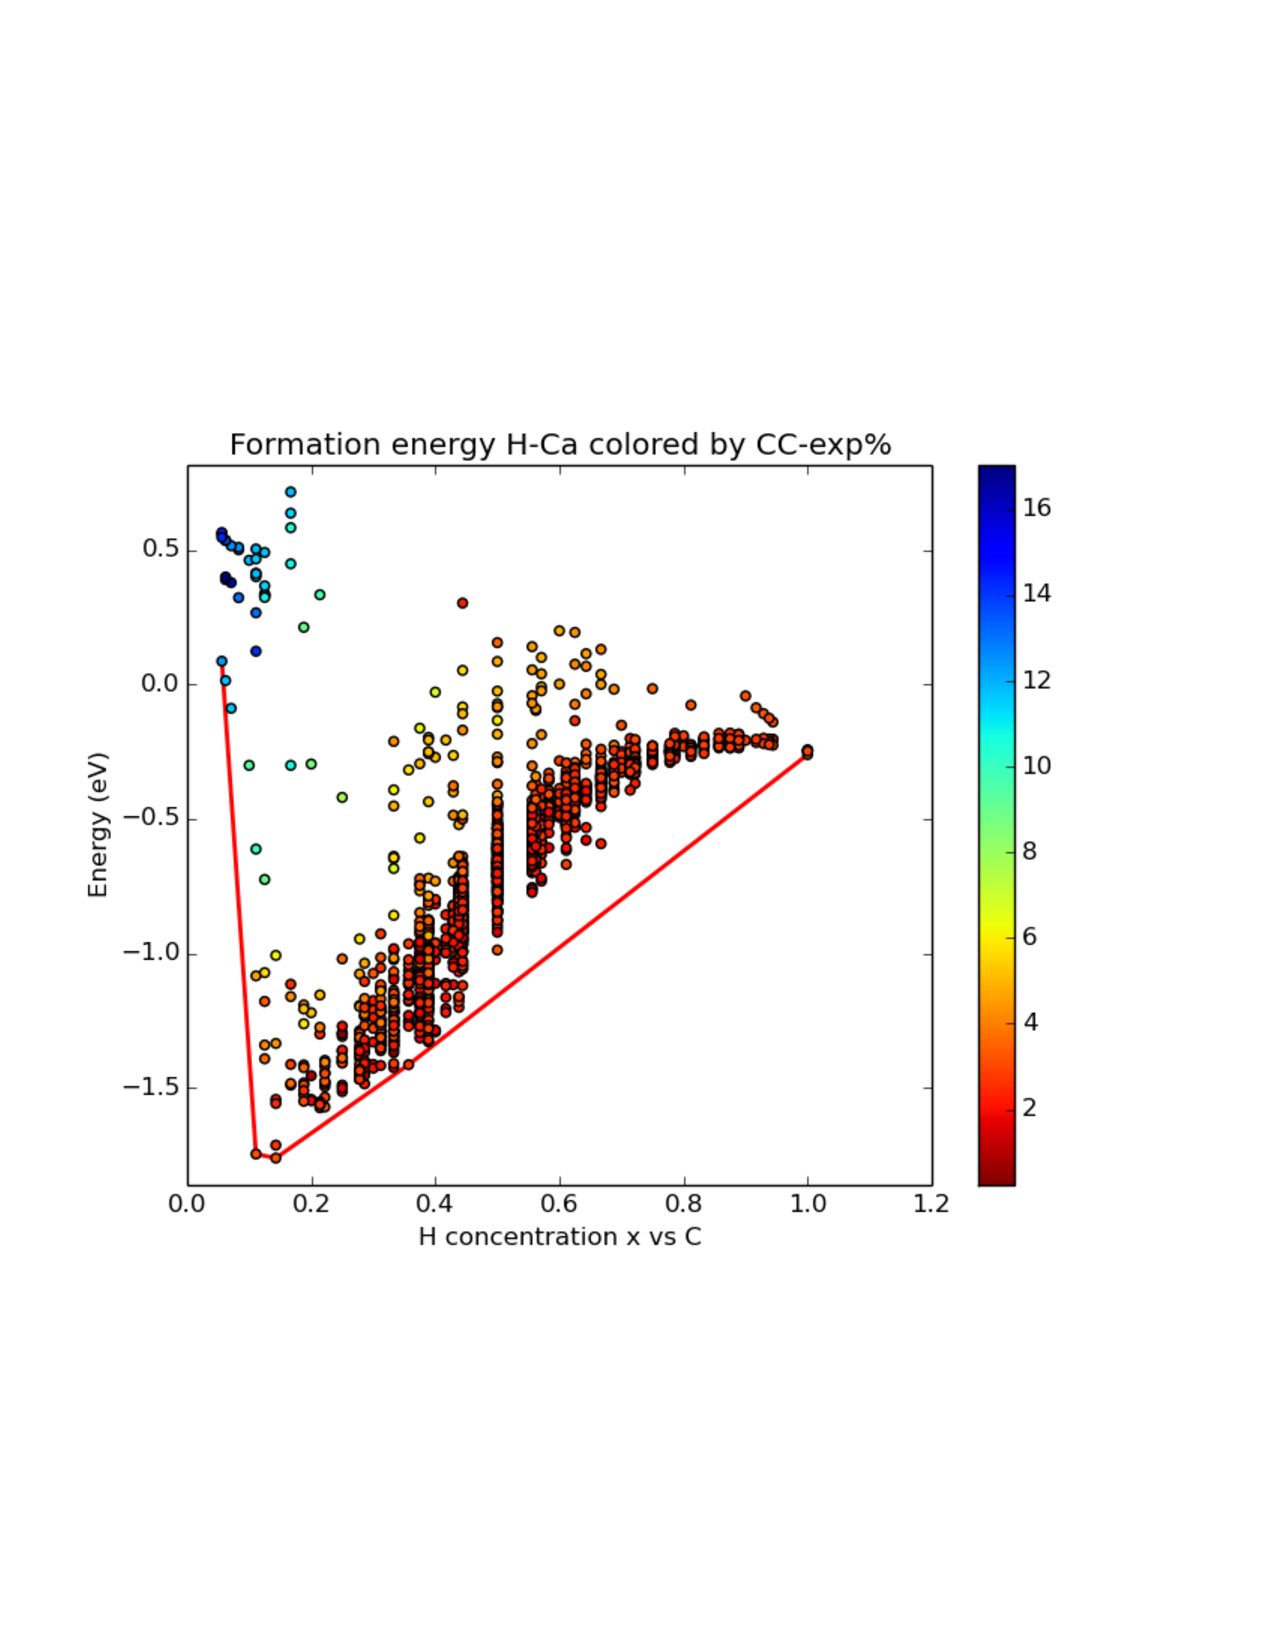
\includegraphics[width=\textwidth]
			{bin_both_FE_CC-exp(atoms0-1)_1} \\
		\textit{(a)}	
	\end{minipage}
	\hfill
	\begin{minipage}{0.49\textwidth}
		\centering
		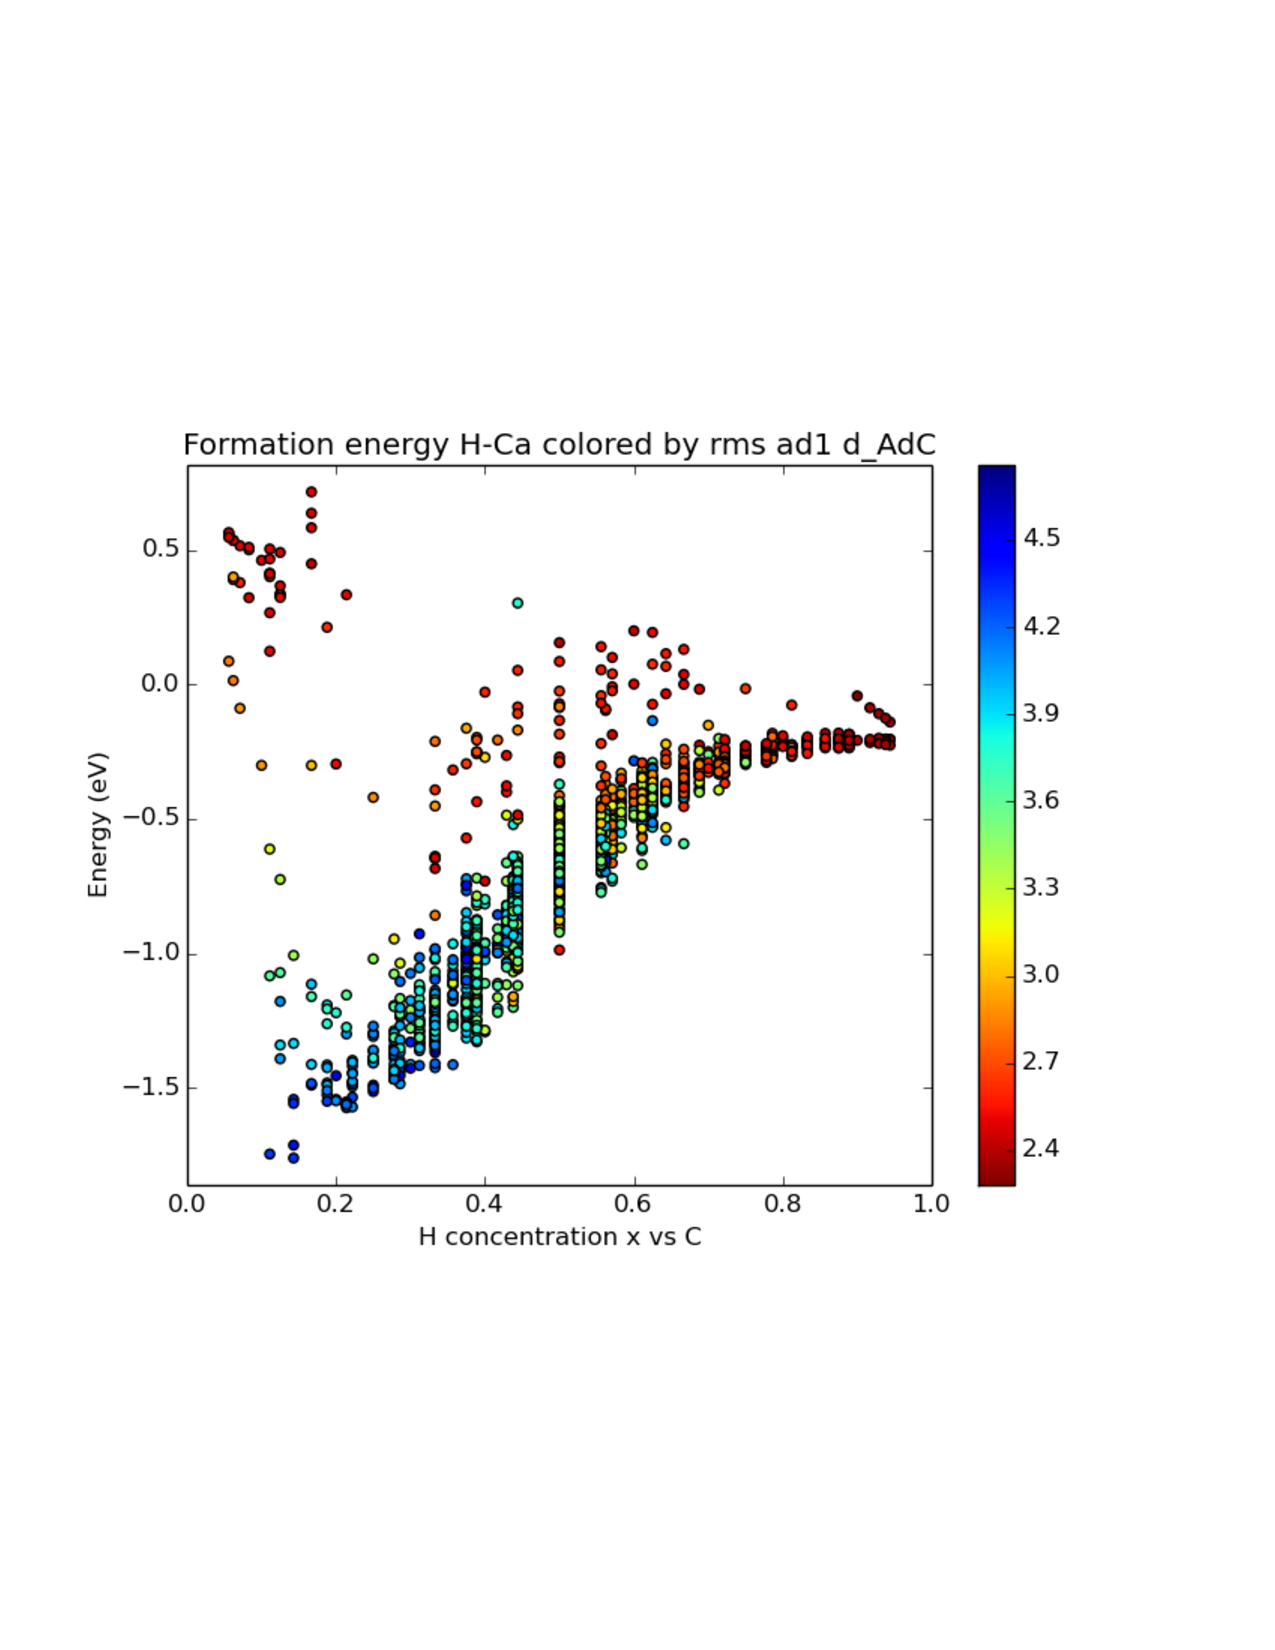
\includegraphics[width=\textwidth]
			{bin_both_FE_rms_ad1_d_AdC(atoms0-1)_1} \\
		\textit{(b)}	
	\end{minipage}
	\caption[Binary Double-Sided Search Data]{A plot of formation 
		energies demonstrating the error in energy calculations. 
		All structures at full hydrogen concentration (graphane) 
		should have the same FE, but this plot shows that there is 
		a spread in the energy values. This spread acts as an error 
		estimate for any energy calculation in the search.}
	\label{bin_both_convex_hull}
\end{figure}

\section{Effect of Vacancies}

We have found it unlikely that any promising structures for hydrogen storage would emerge from either of the binary cases, single-sided or double-sided. However, we also study ternary cases in which we allow three bonding options at each carbon site: a hydrogen atom, a calcium atom, or a vacancy. We find that allowing vacancies in our structure acheives higher calcium concentrations without stacking effects. 

We assume that the error in the energy calculations for ternary cases is similar to the error that was found in the binary cases and we only pay attention to structures that are within that error ($\sim20~meV$) of the lowest calculated structure at each concentration. We can then easily identify at what concentration the calcium atoms begin to bond with each other and isolate from the graphene monolayer. 

For the single-sided case, we were able to find stable structures with calcium concentrations as high as $25~\%$ without stacking whereas stacking was always an issue in the binary case. The most stable structure with a $25~\%$ calcium concentration ($\mathrm{FE} = -2.15~eV$ and $\mathrm{PBE} = -0.743~eV$) is pictured in Figure \ref{tern_top_250_struct}. There are, of course, other stable structures in configurations with less calcium, but we are choosing to focus on structures with high calcium concentration since we believe that they will have higher hydrogen storage capacity.

\begin{figure}
	\centering
	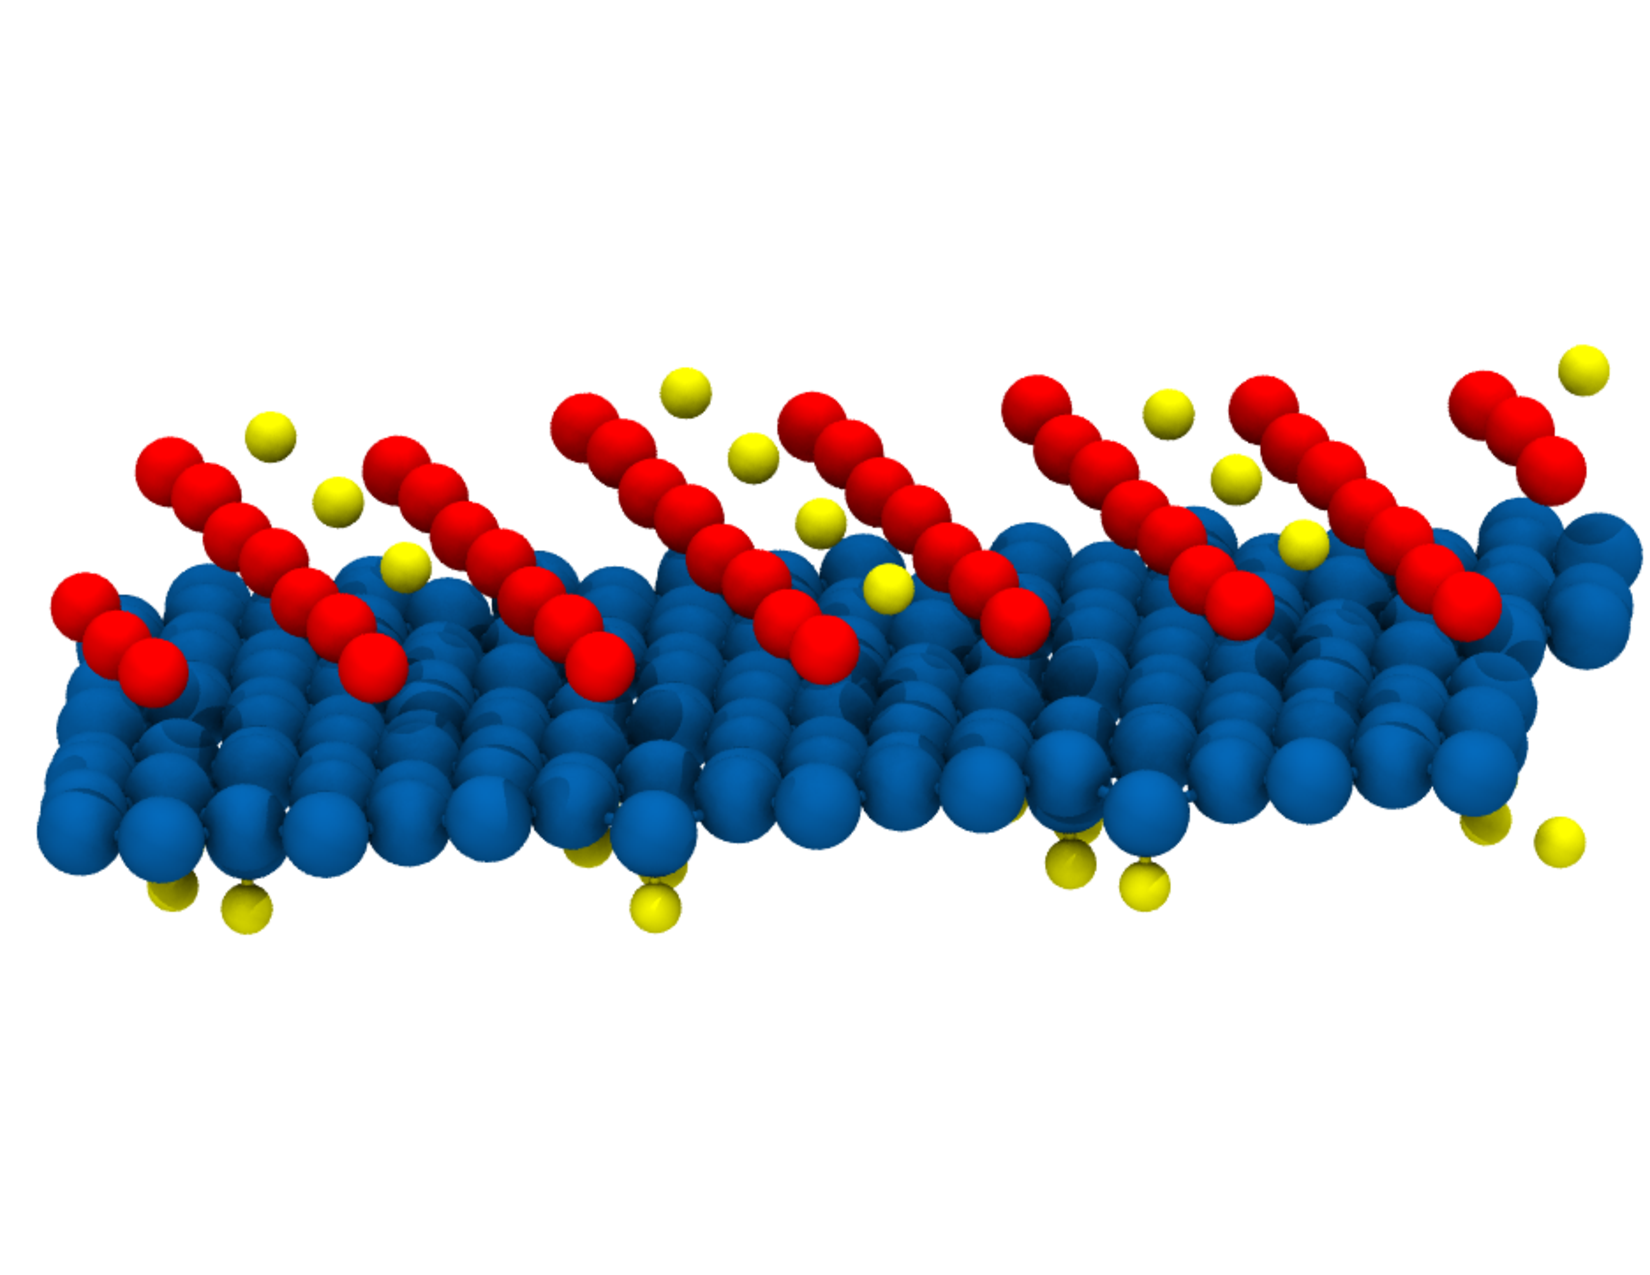
\includegraphics[width=0.6\textwidth]{tern_top_250_struct}
	\caption[Stable Ternary Single-Sided Structure]{The most 
		stable, single-sided structure with a calcium concentration 
		of 25~\%. Because of its stability and high calcium 
		concentration, this structure shows great promise for 
		hydrogen storage applications.}
	\label{tern_top_250_struct}
\end{figure}

For the double-sided case we found structures up to $43.8~\%$ calcium concentration without stacking---a considerable improvement over the binary double-sided case. The most stable double-sided structure with that calcium concentration ($\mathrm{FE} = -1.981~eV$ and $\mathrm{PBE} = -0.199~eV$) is pictured in Figure \ref{tern_both_438_struct}. One intriguing fact about this structure is the fact that there are calcium atoms on both sides of the plane. Double-sided structures have the possibility of utilizing both sides of the plane for hydrogen storage and, therefore, are even more desirable than just single-sided structures.

\begin{figure}
	\centering
	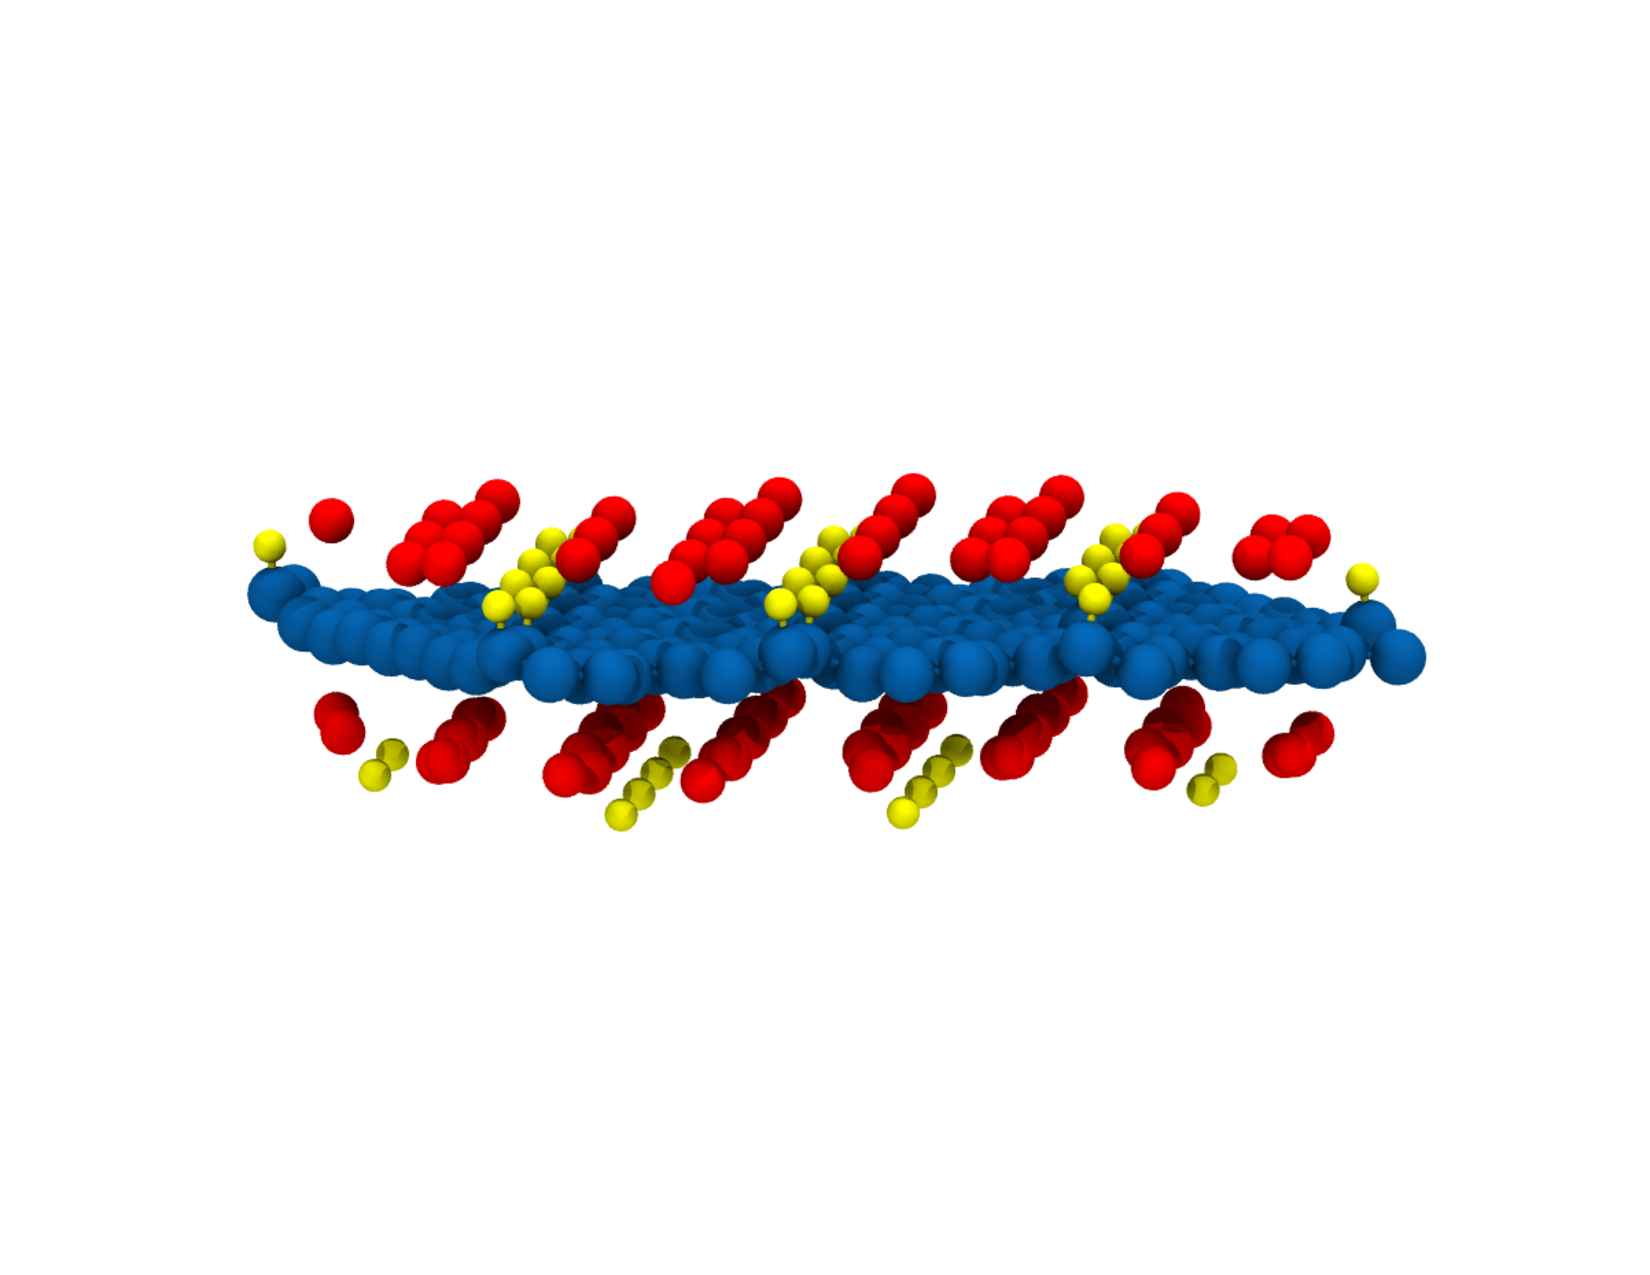
\includegraphics[width=0.6\textwidth]{tern_both_438_struct}
	\caption[Stable Ternary Double-Sided Structure]{The most 
		stable, double-sided structure with a calcium concentration 
		of 43.8~\%. This structure has a lot of calcium on both 
		sides of the plane and, therefore, should be a good 
		candidate for hydrogen storage.}
	\label{tern_both_438_struct}
\end{figure}

The comparisons made above show that vacancies play an important role in the formation of structures for hydrogen storage. We have shown that vacancies allow for significantly higher concentrations of calcium atoms without giving way to stacking. This is a desirable characteristic because, theoretically, structures with a higher concentration of calcium should be able to bind more hydrogen and, therefore, be better suited to hydrogen storage applications.

\section{Variation of Unit Cells}

As mentioned in Section \ref{sec:our_project}, one of our objectives in this project was to expand our search by using a number of different computational unit cell shapes and sizes. It is clear that cell size and shape is an important parameter in the search for low energy structures. 

For example, a full enumeration up through volume nine structures was performed for the binary double-sided case. Only 2,896 of 57,499 total distinct structures were of the traditional $3 \times 3$ unit cell type pictured in Figure \ref{fig:unit_cells} \textit{(d)}. In fact, the overwhelming majority of the structures we were interested in were not of that cell type. This result suggests that the periodicities encompassed by the volume nine, $3 \times 3$ unit cell may not be ideal periodicities for a H-Ca system. In any case, it is an important illustration of the fact that, in order to perform a complete search of the space, the size and shape of the unit cell must be a parameter in the search.

\begin{comment}
% Uncomment this section for appendices.
% Start labeling chapters with letters and calling them appendices
\begin{appendices}

\chapter{Appendix Title}
\label{sec:appendixname}

You can put supplimentary content in an appendix.

\end{appendices}
\end{comment}

% Make the bibliography.
% Enter your references in the BibTex file "references.bib"
\bibliography{references}

% Make the index
 \printindex

\end{document}
